% =====================================================================
%  ChicagoDoes Capstone Paper
%  Personalized Location Recommendation System for ChicagoDoes
%  University of Chicago - MScA Capstone, Spring 2026
%  Formatted to the MScA Capstone Paper Requirements Guide.
% =====================================================================
\documentclass[12pt,letterpaper]{article}

% --- Layout --------------------------------------------------------------
\usepackage[margin=1in]{geometry}
\usepackage{setspace}
\doublespacing
% Indent first line of every paragraph (except Abstract, handled inline).
\setlength{\parindent}{0.5in}
\setlength{\parskip}{0pt}
\usepackage{microtype}
\usepackage{indentfirst}

% --- Typography: Times New Roman ----------------------------------------
\usepackage[T1]{fontenc}
\usepackage{mathptmx}
\usepackage{textcomp}

% --- Math / symbols ------------------------------------------------------
\usepackage{amsmath,amssymb,amsfonts}
\usepackage{bm}
\usepackage{mathtools}

% --- Graphics / tables ---------------------------------------------------
\usepackage{graphicx}
\graphicspath{{./figures/}}
\usepackage{booktabs}
\usepackage{array}
\usepackage{tabularx}
\usepackage{float}
\usepackage{makecell}
\renewcommand\theadfont{\bfseries}

% --- Captions: bold label + italic description, above figure/table ------
\usepackage{caption}
\captionsetup{labelfont=bf,textfont=it,labelsep=period,
  justification=centering,singlelinecheck=false,
  font={small},skip=4pt}
\captionsetup[table]{position=above}
\captionsetup[figure]{position=above}

% --- Color and links -----------------------------------------------------
\usepackage[table]{xcolor}
\definecolor{tableheader}{HTML}{e6ecf4}
\usepackage[
  colorlinks=true,
  linkcolor=black,
  urlcolor=blue!50!black,
  citecolor=black,
  pdftitle={Personalized Location Recommendation System for ChicagoDoes},
  pdfauthor={ChicagoDoes Capstone Team},
]{hyperref}

% --- Section headings (Guide-specified) ---------------------------------
% H1 (section):     14pt bold, centered, Title Case
% H2 (subsection):  12pt bold, left, Title Case
% H3 (subsubsection): 12pt bold italic, left, Title Case
\usepackage{titlesec}
\titleformat{\section}
  {\normalfont\fontsize{14}{17}\selectfont\bfseries\filcenter}
  {}{0pt}{}
\titleformat{\subsection}
  {\normalfont\fontsize{12}{15}\selectfont\bfseries\filright}
  {}{0pt}{}
\titleformat{\subsubsection}
  {\normalfont\fontsize{12}{15}\selectfont\bfseries\itshape\filright}
  {}{0pt}{}
\titlespacing*{\section}{0pt}{12pt}{6pt}
\titlespacing*{\subsection}{0pt}{10pt}{4pt}
\titlespacing*{\subsubsection}{0pt}{8pt}{3pt}

% Guide: "Do not number sections."
\setcounter{secnumdepth}{-1}

% --- Lists ---------------------------------------------------------------
\usepackage{enumitem}
\setlist{itemsep=2pt,topsep=3pt,parsep=0pt}

% --- Page numbering: centered at bottom; no header ----------------------
\usepackage{fancyhdr}
\fancypagestyle{frontmatter}{%
  \fancyhf{}\renewcommand{\headrulewidth}{0pt}%
  \fancyfoot[C]{\thepage}}
\fancypagestyle{body}{%
  \fancyhf{}\renewcommand{\headrulewidth}{0pt}%
  \fancyfoot[C]{\thepage}}

% --- Convenience macros --------------------------------------------------
% Allow line breaks inside long monospace tokens at underscores so that
% identifiers like "is_favorite_location" or "events_intraday_YYYYMMDD"
% do not overflow the right margin.
\newcommand{\codeunderscore}{\discretionary{\textunderscore}{}{\textunderscore}}
\newcommand{\code}[1]{\begingroup\let\_\codeunderscore\texttt{\small #1}\endgroup}
\sloppy
\emergencystretch=3em

% --- TOC formatting: dotted leaders, no L3 -----------------------------
\usepackage{tocloft}
\renewcommand{\cftsecleader}{\cftdotfill{\cftdotsep}}
\renewcommand{\contentsname}{Table of Contents}
\renewcommand{\listfigurename}{List of Figures}
\renewcommand{\listtablename}{List of Tables}
\renewcommand{\cftsecfont}{\normalfont}
\renewcommand{\cftsubsecfont}{\normalfont}
\renewcommand{\cftsecpagefont}{\normalfont}
\setlength{\cftbeforesecskip}{2pt}
\setlength{\cftbeforesubsecskip}{1pt}
\setcounter{tocdepth}{2}

% Centered, bold, 14pt headings for TOC/LoF/LoT (match Level 1).
\renewcommand{\cfttoctitlefont}{\hfill\fontsize{14}{17}\selectfont\bfseries}
\renewcommand{\cftaftertoctitle}{\hfill}
\renewcommand{\cftloftitlefont}{\hfill\fontsize{14}{17}\selectfont\bfseries}
\renewcommand{\cftafterloftitle}{\hfill}
\renewcommand{\cftlottitlefont}{\hfill\fontsize{14}{17}\selectfont\bfseries}
\renewcommand{\cftafterlottitle}{\hfill}

% =====================================================================
\begin{document}

% --- Title page (no page number) ----------------------------------------
\begin{titlepage}
  \thispagestyle{empty}
  \centering
  \vspace*{1.4in}

  {\fontsize{18}{22}\selectfont\bfseries
   Personalized Location Recommendation System\\
   for ChicagoDoes\par}
  \vspace{0.4in}

  {\fontsize{12}{14}\selectfont By\par}
  \vspace{6pt}
  {\fontsize{12}{14}\selectfont Yiou Wang\par}
  {\fontsize{12}{14}\selectfont RJ Xia\par}
  {\fontsize{12}{14}\selectfont Kennedy Damtse\par}
  \vspace{6pt}
  {\fontsize{12}{14}\selectfont Supervisor: Sanjay Boddhu\par}

  \vspace{0.6in}

  {\fontsize{14}{17}\selectfont A Capstone Project\par}
  \vspace{4pt}
  {\fontsize{14}{17}\selectfont Submitted to the University of Chicago in partial fulfillment\par}
  \vspace{4pt}
  {\fontsize{14}{17}\selectfont of the requirements for the degree of\par}
  \vspace{4pt}
  {\fontsize{14}{17}\selectfont Master of Science in Applied Data Science\par}
  \vspace{4pt}
  {\fontsize{14}{17}\selectfont Division of Physical Sciences\par}
  \vspace{4pt}
  {\fontsize{14}{17}\selectfont Summer 2026\par}

  \vfill
\end{titlepage}

% =====================================================================
% Front matter: Roman numerals, centered bottom.
\pagenumbering{roman}
\setcounter{page}{1}
\pagestyle{frontmatter}

% --- Abstract -----------------------------------------------------------
\section*{Abstract}
\noindent
ChicagoDoes is an interactive city-discovery map developed with Ateema
that surfaces Chicago restaurants, attractions, parks, and venues. The
platform presents an identical experience to every visitor despite
collecting rich GA4 behavioral telemetry. This capstone designed and
deployed a personalized location-recommendation system that converts
those events into a weighted hybrid ranker combining content
similarity, item--item and user--user collaborative filtering, session
co-visitation, transition graphs, and event-time trending, with
Maximal Marginal Relevance diversification and behavioral-archetype
cold-start handling. A leakage-safe offline evaluation over 120
returning users benchmarked the ranker against popularity,
content-only, and collaborative baselines; a weight search validated
by five-fold cross-validation improved held-out NDCG@10 by roughly
20 percent. The interface was redesigned around media-rich cards
whose photographs and listing links are scraped with Firecrawl, and
a feedback-loop guard keeps recommender-driven clicks from
re-entering the training data as organic engagement.

\vspace{1in}
\noindent\textit{Keywords}: recommendation systems, hybrid recommender,
collaborative filtering, TF--IDF, implicit feedback, Maximal Marginal
Relevance, cold-start, offline evaluation, tourism analytics, GA4.

\vfill
\newpage

% --- Executive summary --------------------------------------------------
\section*{Executive Summary}

ChicagoDoes faces a personalization gap: visitors browse the same
generalized map regardless of interests, limiting content discovery
and reducing visibility for paying business partners. This capstone
operationalized the GA4 event stream into a recommendation framework
that ranks locations for each visitor and explains every suggestion
with warehouse-backed evidence. A layered BigQuery warehouse converts
raw GA4 events into qualified user--location interactions, aggregated
features, and a full candidate set. On top of the warehouse, a hybrid
recommender blends six signals: TF--IDF content similarity over
location categories, leakage-safe global popularity priors, item--item
Jaccard co-visitation, user--user $k$-nearest-neighbor collaborative
scores, event-time trending, and session co-visitation with a
previous-to-next transition graph. Maximal Marginal Relevance
re-ranking enforces diversity, and cold-start users are served via a
form-derived pseudo-profile and a category-based archetype assignment
from $K$-Means clustering. The system is delivered as a FastAPI
backend and a JavaScript frontend with an optional LLM concierge layer
restricted to the deterministic recommendation pool. Descriptive
analysis confirmed three design choices: popularity must be measured
by distinct users, map-marker clicks and detail call-to-action events
are the cleanest engagement signals, and session-level co-visitation
dominates user-level co-visitation given the prevalence of
single-session users. An offline evaluation harness with a
leave-last-one temporal split scored the ranker on 120 returning
users against popularity, content-only, and collaborative baselines;
a search over more than 4{,}000 weight configurations, validated
with five-fold cross-validation and tracked in MLflow, improved
held-out NDCG@10 by roughly 20 percent and quantified that MMR
trades about 6 percent of ranking accuracy for more than double the
intra-list diversity. The interface was redesigned around media-rich
recommendation cards with Firecrawl-scraped venue photography, each
linking to the venue's ChicagoDoes listing page, and a feedback-loop
guard tags and separately logs these outbound clicks so
recommender-driven traffic does not re-enter the training data as
organic engagement. Online A/B testing, identity linking for
the returning-user path, and retrieval-augmented generation are
scoped as the next deployment phase.

\newpage

% --- Table of contents, List of Figures, List of Tables -----------------
\setcounter{tocdepth}{2}
\tableofcontents
\listoffigures
\listoftables
\newpage

% =====================================================================
% Body: Arabic numerals, reset to 1.
\pagenumbering{arabic}
\setcounter{page}{1}
\pagestyle{body}

\section{Introduction}\label{sec:intro}

\subsection{Problem Statement}\label{sec:problem}

Digital tourism and location-discovery platforms have become a primary
channel through which visitors evaluate where to eat, stay, and
explore. Despite the volume of behavioral data such platforms collect,
many city-exploration products still present an identical browsing
experience to every user. ChicagoDoes, an interactive map developed in
collaboration with Ateema that showcases Chicago restaurants,
attractions, bars, museums, parks, theaters, sports venues, and
entertainment experiences, exhibits this gap. The platform serves
marketing campaigns, links, and embedded QR codes for businesses that
pay for placement, so location visibility and user engagement translate
directly into commercial outcomes for both Ateema and its partners.

ChicagoDoes already collects substantial volumes of map-interaction
telemetry through Google Analytics 4 (GA4): map-marker clicks, page
views, category filters, location searches, media-gallery interactions,
scrolling behavior, and engagement with call-to-action (CTA) elements.
None of this signal is currently operationalized into a personalization
layer. Every visitor, whether interested in nightlife, family-friendly
museums, or outdoor parks, receives the same default browsing
experience. The opportunity is therefore twofold: close a content
discovery gap that limits how many relevant locations each user
encounters, and capture commercial upside for paying partners by
increasing the probability that their venues are shown to users with
matching interests.

The cost of inaction is measurable. With every additional session that
ends without meaningful engagement, ChicagoDoes loses an opportunity
to retain a visitor, drive a partner CTA click-through, or build the
longitudinal behavioral record needed for stronger personalization in
the future. The client's desired solution is a scalable recommendation
framework that converts the existing GA4 data into a personalized,
explainable, and continuously improvable layer on top of the existing
map experience, benefiting both visitors and the businesses featured
on the platform.

\subsection{Analysis Goals}\label{sec:goals}

This capstone designed, built, and operationalized a personalized
location-recommendation system for ChicagoDoes by leveraging GA4
interaction signals together with the platform's location and category
metadata. The system was intended to operate as a production-grade
recommendation layer that improves engagement, supports content
discovery, and establishes the data infrastructure required for future
personalization work. The objectives were to translate raw GA4 event
logs into a layered, queryable warehouse exposing user--location
interactions and full user-by-location candidate pairs; engineer
leakage-safe predictive features at the user and location level;
implement a hybrid recommender that combines content-based similarity,
item--item and user--user collaborative filtering, session-level
co-visitation, transition-graph signals, and event-time trending;
handle cold-start visitors through a form-driven onboarding profile
and behavioral-archetype assignment derived from $K$-Means clustering;
ensure recommendations are diverse by applying Maximal Marginal
Relevance (MMR) re-ranking; deliver a working full-stack web
application (FastAPI backend, JavaScript frontend) demonstrating the
recommender end-to-end with evidence and verified venue media for
every recommendation; evaluate the ranker offline with standard
implicit-feedback ranking metrics (Precision@K, Recall@K, NDCG)
against simpler baselines and tune the score-blend weights under
cross-validation; protect the integrity of the client's behavioral
data by preventing recommender-driven clicks from feeding back into
the training signal; and specify an online A/B methodology to guide
subsequent iterations.

\subsection{Scope}\label{sec:scope}

The work was bounded along five dimensions. First, the model was
trained and evaluated exclusively on ChicagoDoes locations within
Chicago, so transferability to other cities or platforms is plausible
but not validated. Second, behavioral data was restricted to the GA4
event stream collected during the study window (early 2026 onward),
so long-term seasonality and inter-year trends cannot be modeled from
this snapshot alone. Third, the implementation operated on implicit
feedback (clicks, dwell time, qualified engagement events); explicit
ratings and post-visit feedback were not available. Fourth, the LLM
concierge layer was treated as a wrapper around the deterministic
recommendation pool; the language model never injects new locations
and never overrides the underlying ranking. Fifth, quantitative
evaluation was restricted to offline analysis: ranking accuracy was
measured on held-out interactions of 120 returning users under a
temporal split, and the protocol does not yet cover cold-start
visitors. Online experimentation with live traffic remained out of
scope and is specified as a methodology for the next deployment
phase.

% =====================================================================
\section{Background}\label{sec:background}

Ateema is a digital experience company that builds interactive map and
content platforms for destination marketing organizations and city
tourism partners. The capstone focused on its ChicagoDoes property, a
Mapme-backed interactive video map showcasing Chicago's hospitality,
entertainment, and cultural venues. Visitors typically reach the
platform through tourism campaigns, partner links, hotel concierge QR
codes, and embedded marketing assets. Businesses and venues, including
restaurants, tour operators, hotels, museums, parks, and bars, pay for
placement and promotion on the map, making the platform's ability to
drive engaged, category-relevant traffic a direct revenue lever.

Behaviorally, a ChicagoDoes session begins when a user loads the map
(\code{map-load}). The user can then zoom and pan, click category
filters (\code{single-cat-filter}), open a list panel, click an
individual map marker (\code{map-marker-click}), scroll through
location media, and tap CTA buttons such as
\code{section-details-call-to-action}. Each interaction is captured
through GA4 and exposed through BigQuery as event-level records with
payload metadata that ties an event back to a specific location or
category. Despite this instrumentation, the platform's user-facing
surface remains generic. There is no personalization layer that
ingests these events, infers user preferences, and ranks the location
set accordingly. This capstone built that missing layer, grounded it
in the existing warehouse, and delivered it as a deployable web
service.

\subsection{Literature Review}\label{sec:lit}

Recommendation systems have evolved substantially over the past two
decades, with the literature documenting a clear progression from
simple memory-based methods to deep neural and hybrid architectures
(Aggarwal, 2016; Ricci et~al., 2015). Early collaborative filtering
relied on user--user or item--item similarity computed from explicit
ratings, while later work introduced matrix factorization techniques
such as Singular Value Decomposition and Alternating Least Squares
(Koren et~al., 2009). For implicit-feedback scenarios, which closely
match the ChicagoDoes setting where the only signal is whether and how
strongly a user interacted with a location, Hu, Koren, and Volinsky
(2008) proposed weighted matrix factorization with confidence-weighted
positive observations, which became foundational in industrial
recommender systems.

Content-based methods (Pazzani \& Billsus, 2007) take a complementary
approach: each item is represented by feature vectors derived from its
attributes (text descriptions, categories, tags), and items are scored
by similarity to the user's profile. TF--IDF (Salton \& Buckley, 1988)
remains a standard baseline for representing text or categorical
content and is particularly suitable for cold-start environments where
new items have known attributes but few interactions.

Hybrid recommenders, which combine collaborative and content-based
signals, consistently outperform single-paradigm systems on diverse
datasets (Burke, 2002; \c{C}ano \& Morisio, 2017). Hybridization is
especially valuable when interaction sparsity is high, a
near-universal condition for early-stage tourism and discovery
platforms, because content features can backstop the ranking when
collaborative signals are insufficient. Burke (2002) provides the
canonical taxonomy of hybridization strategies (weighted, switching,
mixed, feature-combination, cascade, feature-augmentation,
meta-level); the weighted and feature-combination class is the most
common operational pattern in production systems.

Beyond pointwise scoring, two further strands informed the ChicagoDoes
design. Session-aware and sequence-aware recommendation (Hidasi
et~al., 2016; Quadrana et~al., 2018) demonstrates that co-occurrence
within a single session carries far stronger intent than user-level
co-occurrence across sessions, directly motivating the session-Jaccard
and transition-graph terms in the scoring blend. Ranking
diversification, originating with Maximal Marginal Relevance
(Carbonell \& Goldstein, 1998), addresses the well-documented tendency
of relevance-only ranking to produce homogeneous lists; MMR introduces
a tunable diversity weight that balances relevance with novelty and
has become a standard post-processing step in modern industrial
recommenders.

Applications in tourism are well-documented (Borr\'{a}s et~al., 2014;
Gavalas et~al., 2014). Tourism recommenders typically face severe
cold-start problems, since visitors arrive without history and depart
shortly, and frequently rely on a combination of user-supplied
preferences (vibe, traveler type, interests), contextual signals
(location, time of day), and behavioral aggregates (popularity,
trending). Cold-start handling via onboarding forms, demographic
priors, and segmentation is a recurring design pattern in this
literature. Outside the tourism domain, hybrid recommendation has been
deployed at scale in streaming media (Gomez-Uribe \& Hunt, 2015),
e-commerce, news, and music discovery, where the same building blocks,
namely implicit feedback, content vectorization, co-visitation, and
diversity re-ranking, recur. These external applications confirm that
the methodology selected for ChicagoDoes is well-supported,
transferable, and production-grade rather than narrowly academic.
Finally, recent work on retrieval-augmented generation (Lewis et~al.,
2020) and large language models in recommender systems (Wu et~al.,
2024) suggests RAG-style augmentation as a natural extension to the
present deterministic LLM concierge layer.

% =====================================================================
\section{Data}\label{sec:data-section}

\subsection{Data Sources}\label{sec:data-sources}

All data originated from the Ateema BigQuery project
\code{ateema-capstone}, dataset \code{analytics\_459092297}. Three
categories of underlying sources fed the warehouse: raw GA4 daily
event tables (\code{events\_YYYYMMDD} and
\code{events\_intraday\_YYYYMMDD}) exported automatically from the
ChicagoDoes site instrumentation; the official Mapme and Ateema
location and category lists, used as canonical dimensional truth; and
a crawler-derived location--category bridge, cleaned and normalized to
produce the working \code{location\_category\_dim} table. A fourth,
presentation-side source supplements the warehouse: a
Firecrawl-derived enrichment store (\code{data/location\_cards.json})
holding, for each location, photographs and videos scraped from its
ChicagoDoes listing gallery and official website, the resolved
ChicagoDoes listing URL, and corrected geographic coordinates. This
store feeds the user interface only and contributes no modeling
features. A layered
warehouse progressively transformed events into modeling-ready
features (Table~\ref{tab:warehouse}). The principal modeling variables
used by the recommender are summarized in Table~\ref{tab:variables}.

\begin{table}[H]
\centering
\caption{ChicagoDoes data-warehouse layers and their role in the recommender}
\label{tab:warehouse}
\small
\rowcolors{2}{tableheader!40}{white}
\begin{tabularx}{\linewidth}{lXl}
\toprule
\thead[l]{Table} & \thead[l]{Role} & \thead[l]{Used by recommender} \\
\midrule
\code{location\_dim}                  & Official location dimension (canonical names, IDs). & Indirect \\
\code{category\_mapping}              & Official category dimension; modeling vocabulary.   & Indirect \\
\code{location\_category\_bridge\_final} & Cleaned location $\times$ category mapping.      & Indirect \\
\code{location\_category\_dim}        & Normalized location $\times$ category dimension.    & Yes (TF--IDF input) \\
\code{user\_location\_category\_events} & Flattened, parsed GA4 events with location and category. & Yes (behavior, trends) \\
\code{user\_location\_full\_features} & Aggregated (user, location) features and \code{*\_all\_users} priors. & Yes (primary input) \\
\code{candidate\_user\_location\_table} & Full user $\times$ all official locations expansion. & Yes (candidate set) \\
\bottomrule
\end{tabularx}
\end{table}

\begin{table}[H]
\centering
\caption{Principal modeling variables and their role in the hybrid ranking}
\label{tab:variables}
\small
\rowcolors{2}{tableheader!40}{white}
\begin{tabularx}{\linewidth}{lXl}
\toprule
\thead[l]{Variable} & \thead[l]{Type and source} & \thead[l]{Role in ranking} \\
\midrule
Categories (TF--IDF)         & Location-level vector from \code{location\_category\_dim}  & Content similarity $s_\text{sim}$ \\
\code{popularity\_norm}      & Location scalar; \code{*\_all\_users} distinct users        & Popularity prior $s_\text{pop}$ \\
\code{engagement\_norm}      & Location scalar; \code{*\_all\_users} engagement time       & Popularity support \\
\code{is\_hot\_spot\_location} & Location-level flag                                       & Categorical boost \\
\code{is\_favorite\_location} & Location-level flag                                        & Categorical boost \\
Item Jaccard $J(i,j)$        & Sparse matrix from qualified user $\times$ location          & Item--item CF $s_\text{item}$ \\
User category share (L2)     & User-level vector across categories                          & User--user kNN $s_\text{user}$ + archetype \\
Trending norm                & Location scalar from time-split events                       & Trending $s_\text{trend}$ \\
Session Jaccard              & Sparse matrix from session-grouped events                    & Session co-visit (part of $s_\text{sess}$) \\
Transition $P(j\!\mid\!i)$   & Sparse matrix from \code{previous\_location\_id}             & Transition graph (part of $s_\text{sess}$) \\
\code{profile\_weight}       & Per (user, location) weight for behavioral profile           & Profile construction only \\
\bottomrule
\end{tabularx}
\end{table}

The primary unit of analysis was the
$(\text{user\_key}, \text{location\_id})$ pair, augmented with
category vectors at the location level and behavioral category-share
vectors at the user level. Time aggregation operated over the full
GA4 observation window; all global priors were re-aggregated on each
warehouse refresh. Users and events were not subsampled; every
qualified interaction in the warehouse contributed to user-level and
location-level features. An engagement-quality filter
(\code{backend/engagement.py}) down-selected events feeding
collaborative signals by excluding scroll noise, navigation-only
events, and very short page views while up-weighting strong map-user
actions. The filter is configurable through three policies
(\code{permissive}, \code{balanced}, \code{strict}); \code{balanced}
is the production default. Because the recommender operates on
implicit feedback there is no traditional rating-style target. The
implicit positive label for each (user, location) pair was derived
from qualified engagement, while implicit negatives were constructed
via candidate expansion over the user $\times$ all-locations table.
Predictive variables include TF--IDF category vectors, leakage-safe
popularity and engagement priors, hot-spot and favorite flags, item
co-visitation similarities, user--user kNN scores, session
co-visitation similarities, transition-graph next-location
probabilities, and event-time trending ratios. Sparse explicit
feedback, the short observation window, anonymous and
single-session users, missing demographic attributes, the loss of
conversion signal once a user leaves the map, limited
location-content metadata, cold-start locations with no prior
interactions, and the inherent label-leakage risk between aggregated
features and predictive targets are the principal data limitations
that shaped the methodology.

\subsection{Descriptive Analysis}\label{sec:descriptive}

Exploratory data analysis was conducted on the GA4 event stream to
characterize how users actually interact with the map and to validate
design choices for the recommender. Figures~\ref{fig:user_overview}
through~\ref{fig:temporal} summarize the principal findings; the
underlying notebook is \code{EDA.ipynb}.

\begin{figure}[H]
  \centering
  \caption[User overview: daily active users, devices, and geography]{User overview: daily active users, device distribution, and geographic reach (selected weeks, GA4 \code{map-user-action} events)}
  \label{fig:user_overview}
  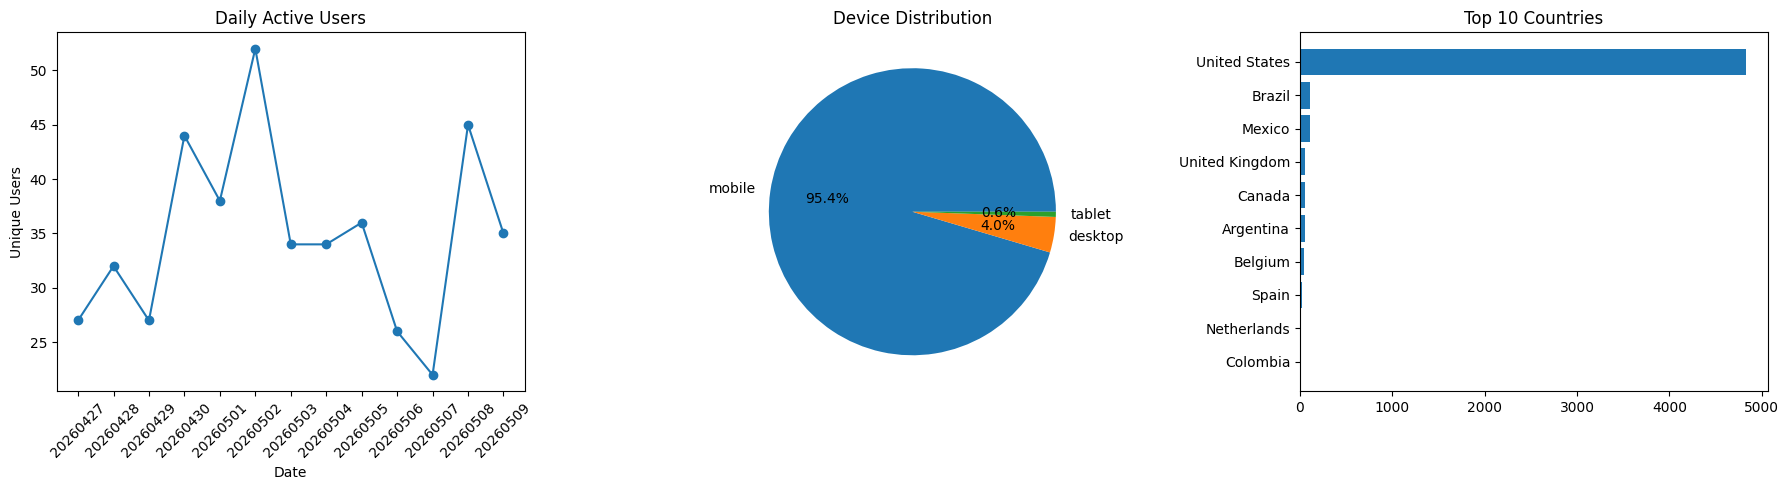
\includegraphics[width=\linewidth]{fig_user_overview.png}
\end{figure}

Daily active users, device distribution, and geographic reach
(Figure~\ref{fig:user_overview}) were computed from the
\code{map-user-action} event population. The user base is
predominantly desktop and concentrated in the United States with
long-tail international traffic from referral campaigns. Daily active
users were non-uniform across the observation window and exhibited
clear weekly seasonality consistent with tourism browsing.

\begin{figure}[H]
  \centering
  \caption{Top 20 listings by total clicks (left) and by unique users (right). The two rankings diverge, revealing repeat-visit-dominated listings}
  \label{fig:listings}
  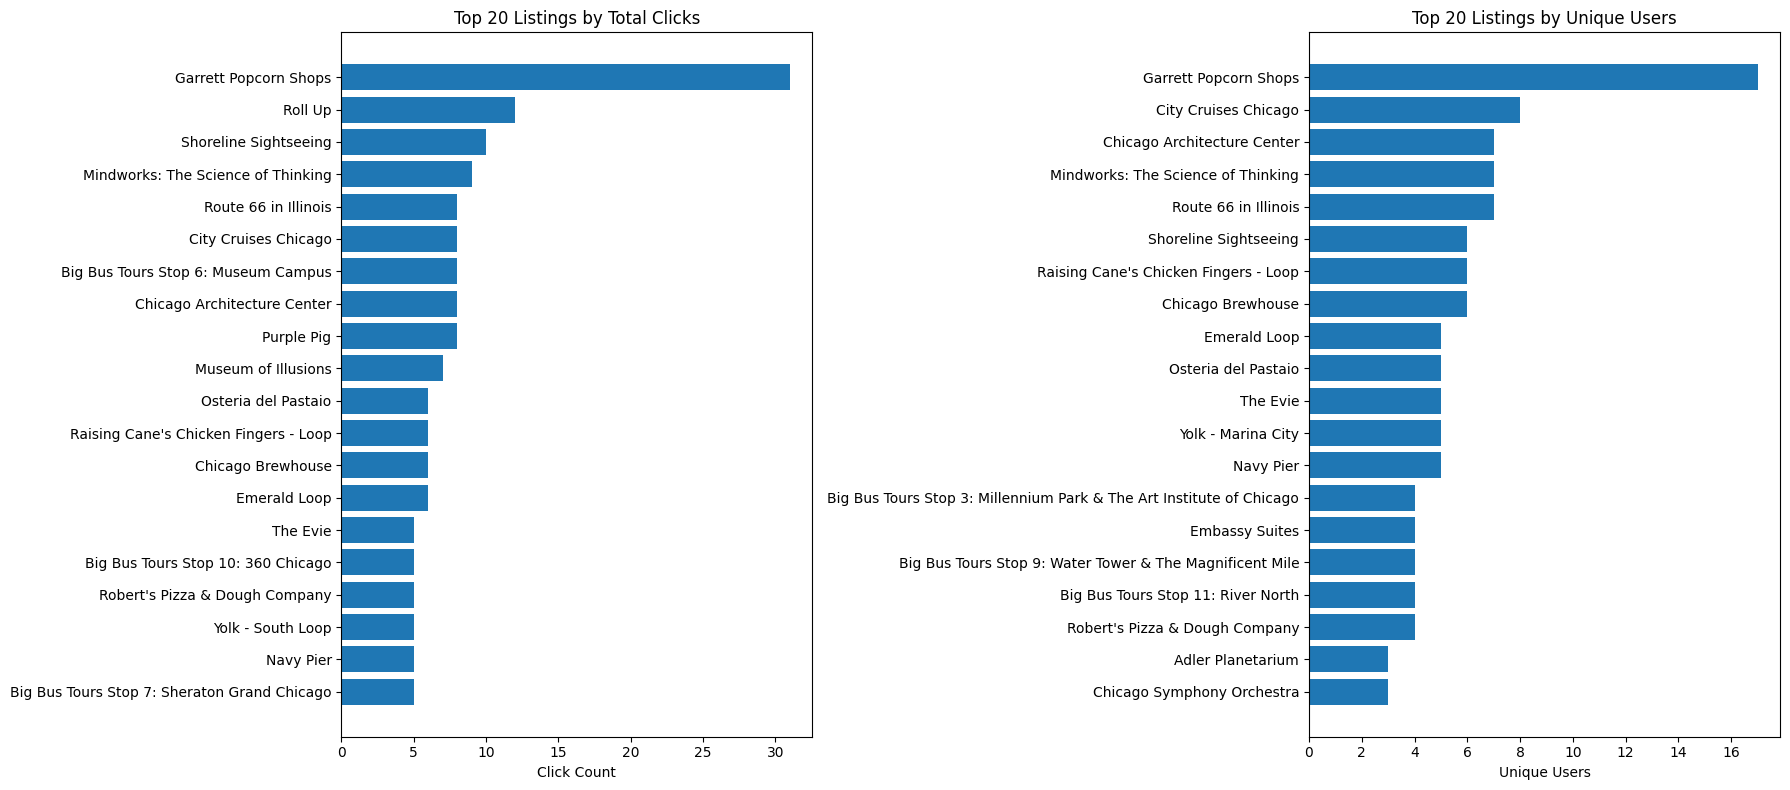
\includegraphics[width=\linewidth]{fig_listing_engagement.png}
\end{figure}

Top listings (Figure~\ref{fig:listings}) were ranked by total clicks
and unique users. Garrett Popcorn Shops led both metrics (31 total
clicks and 17 unique users), making it the single most consistently
popular listing. The second-ranked listing by total clicks, Roll Up,
was concentrated in only two unique users, a pattern indicating
repeated visits by the same person rather than broad appeal. This
finding was operationalized in the recommender: popularity is
computed as \code{popularity\_norm} over distinct users rather than
raw clicks, so high-repeat, low-reach listings are not over-promoted.

\begin{figure}[H]
  \centering
  \caption{User behavior depth: listings per user (left) and breakdown of action types (right)}
  \label{fig:depth}
  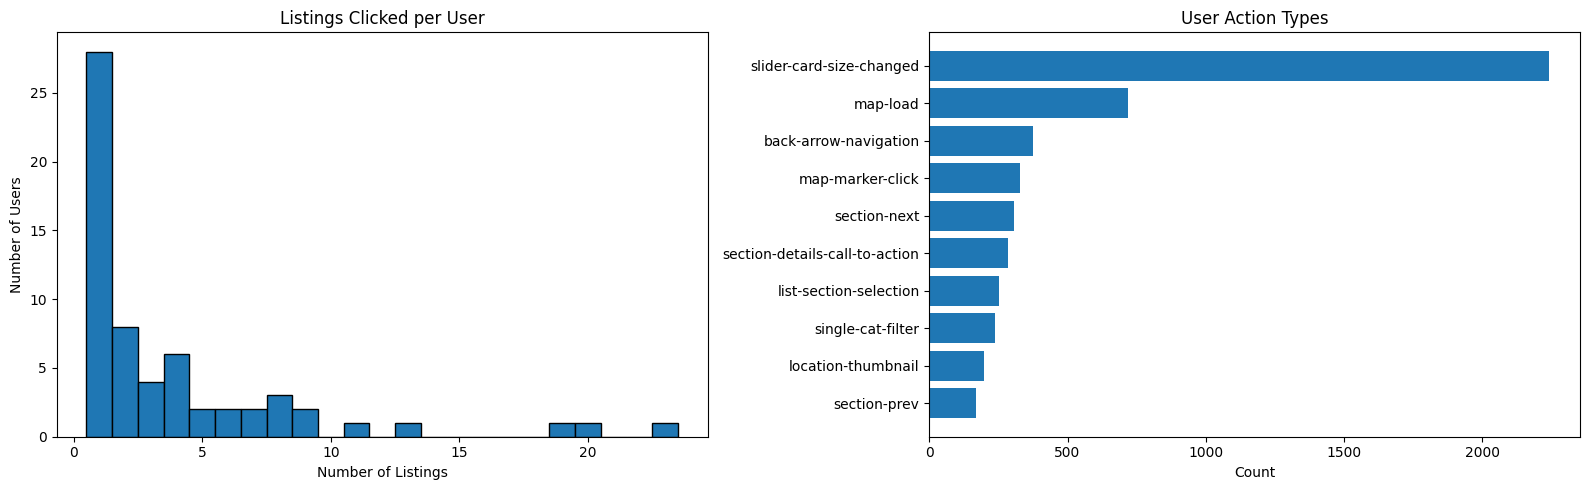
\includegraphics[width=\linewidth]{fig_behavior_depth.png}
\end{figure}

Over half of users clicked only one or two listings per session
(Figure~\ref{fig:depth}), indicating low exploration depth and
reinforcing the need for a recommender that surfaces relevant content
earlier. \code{slider-card-size-changed} dominated raw action volume
but is UI-driven rather than content-intent;
\code{map-marker-click} and \code{section-details-call-to-action}
emerged as the cleanest signals and were classified as
\code{STRONG\_ACTIONS} in \code{backend/engagement.py}.

\begin{figure}[H]
  \centering
  \caption[Engagement funnel: map-load to detail call-to-action]{Engagement funnel: \code{map-load} $\rightarrow$ \code{map-marker-click} $\rightarrow$ \code{section-next} $\rightarrow$ \code{section-details-call-to-action}}
  \label{fig:funnel}
  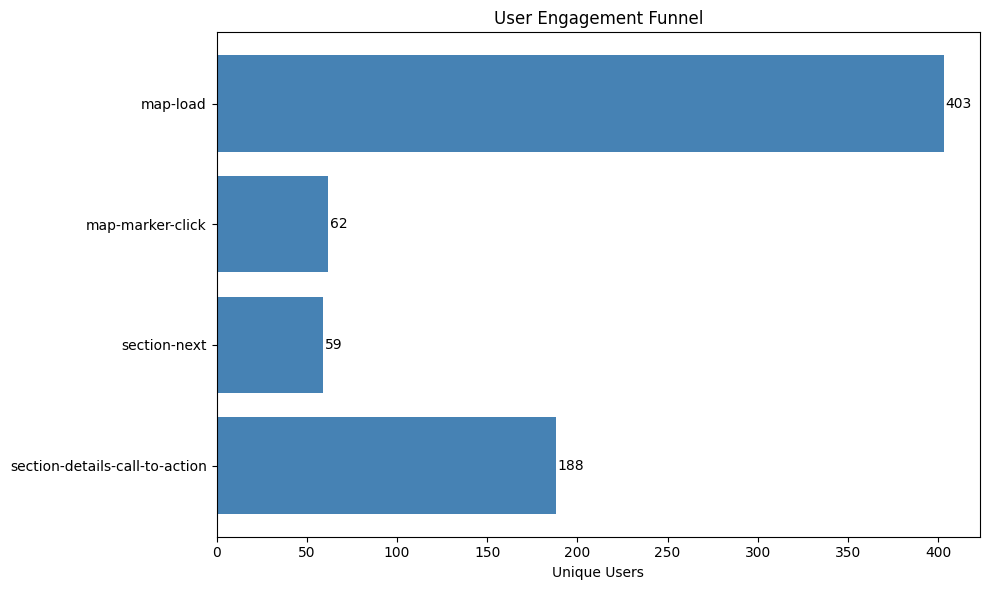
\includegraphics[width=0.85\linewidth]{fig_engagement_funnel.png}
\end{figure}

Of 403 users who loaded the map (Figure~\ref{fig:funnel}), only 62
(15 percent) clicked a specific listing marker. Notably,
\code{section-details-call-to-action} showed 188 users, higher than
\code{map-marker-click}, indicating that many users reach listing
detail pages through paths other than direct marker clicks (list
browsing, category filtering). This pattern validated the decision to
treat list-section selections and CTA clicks as first-class signals.

\begin{figure}[H]
  \centering
  \caption{Entry-point analysis: most common first listing clicked per user session}
  \label{fig:entry}
  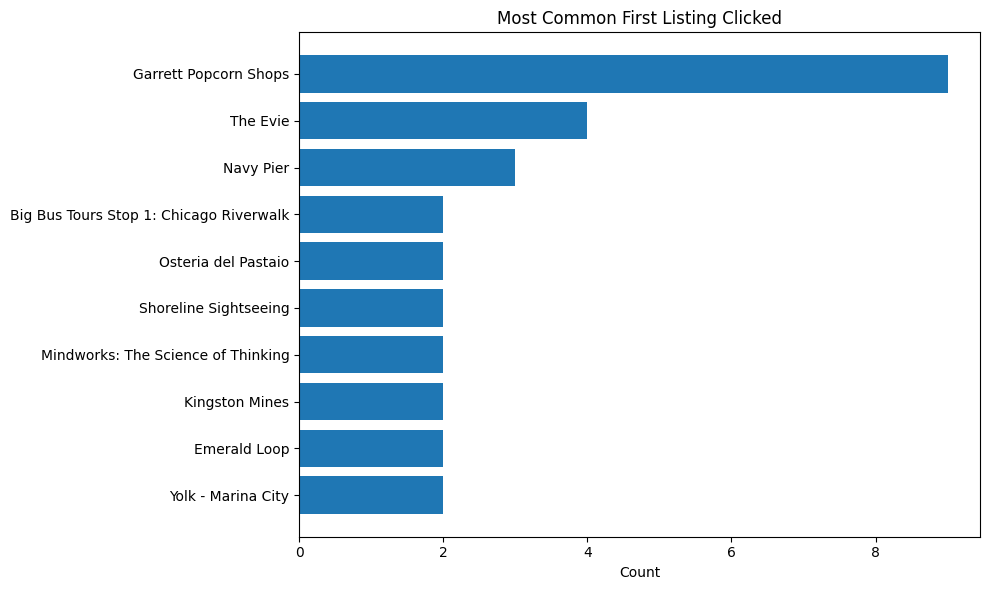
\includegraphics[width=0.95\linewidth]{fig_entry_points.png}
\end{figure}

Garrett Popcorn Shops was by far the most common entry point
(Figure~\ref{fig:entry}), clicked first by 9 users; The Evie (a hotel)
and Navy Pier followed, reflecting two distinct intents,
accommodation seekers and landmark-oriented tourists. The recommender
exploits this divergence through behavioral archetypes
(see Cold-Start Handling and User Archetypes).

\begin{figure}[H]
  \centering
  \caption{Temporal activity patterns: hour-of-day by day-of-week activity}
  \label{fig:temporal}
  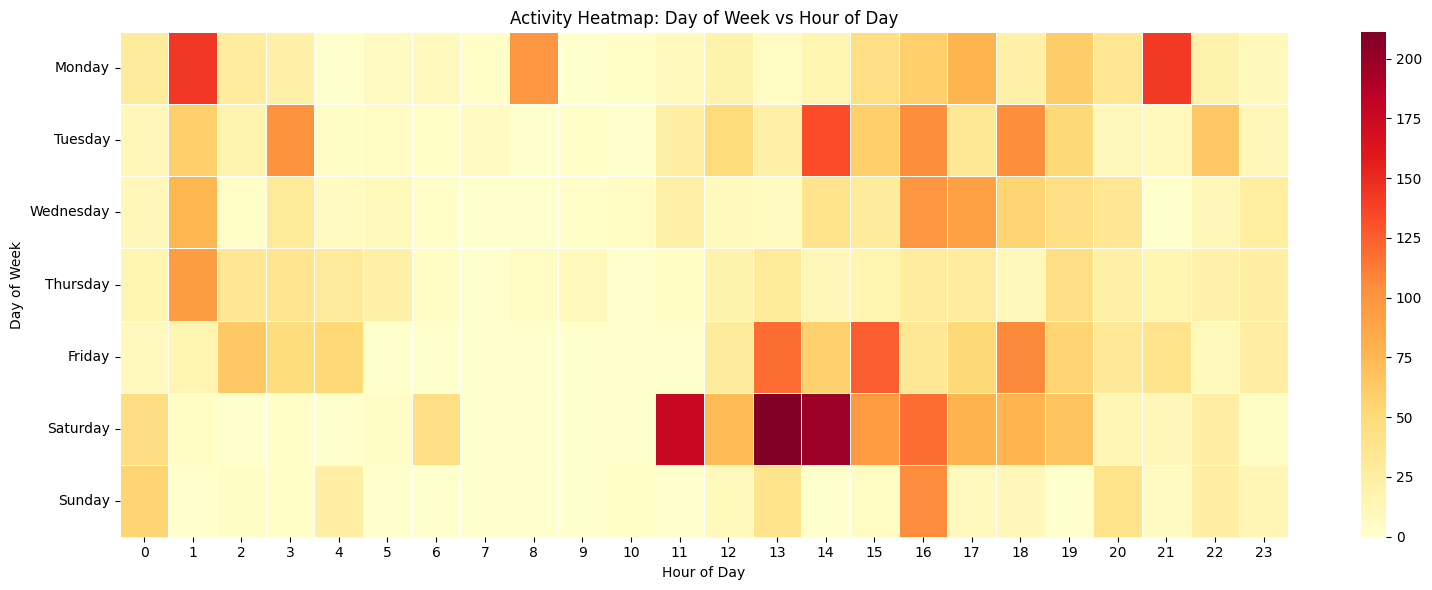
\includegraphics[width=\linewidth]{fig_temporal_activity.png}
\end{figure}

Activity peaked on Saturday between 11~a.m. and 3~p.m.
(Figure~\ref{fig:temporal}), aligning with weekend tourist hours.
Weekday activity was more spread out with notable early-afternoon
spikes. Activity between 3 and 9~a.m. was low across all days,
consistent with typical sleep hours and validating the time-split
logic of the trending signal in \code{backend/trends.py}. Taken
together, the descriptive findings justify three design decisions
carried forward into the methodology: popularity must be measured by
distinct users rather than raw clicks; map-marker clicks and detail
CTA events are the cleanest engagement signals; and session-level
co-visitation is more informative than user-level co-visitation given
the prevalence of single-session users.

% =====================================================================
\section{Methodology}\label{sec:methodology}

The system consists of a layered data warehouse that converts raw GA4
events into modeling-ready features, a hybrid recommender that
combines six complementary scoring signals, cold-start handling via
form-based profiles and behavioral archetypes, a diversity-aware
re-ranking step using MMR, and an LLM concierge layer that operates
only on the deterministic recommendation pool. The end-to-end
architecture is shown in Figure~\ref{fig:arch}.

\begin{figure}[H]
  \centering
  \caption{End-to-end architecture: raw GA4 events transform through the layered warehouse and modeling features into the hybrid ranking engine, which is exposed by a FastAPI application with an LLM concierge}
  \label{fig:arch}
  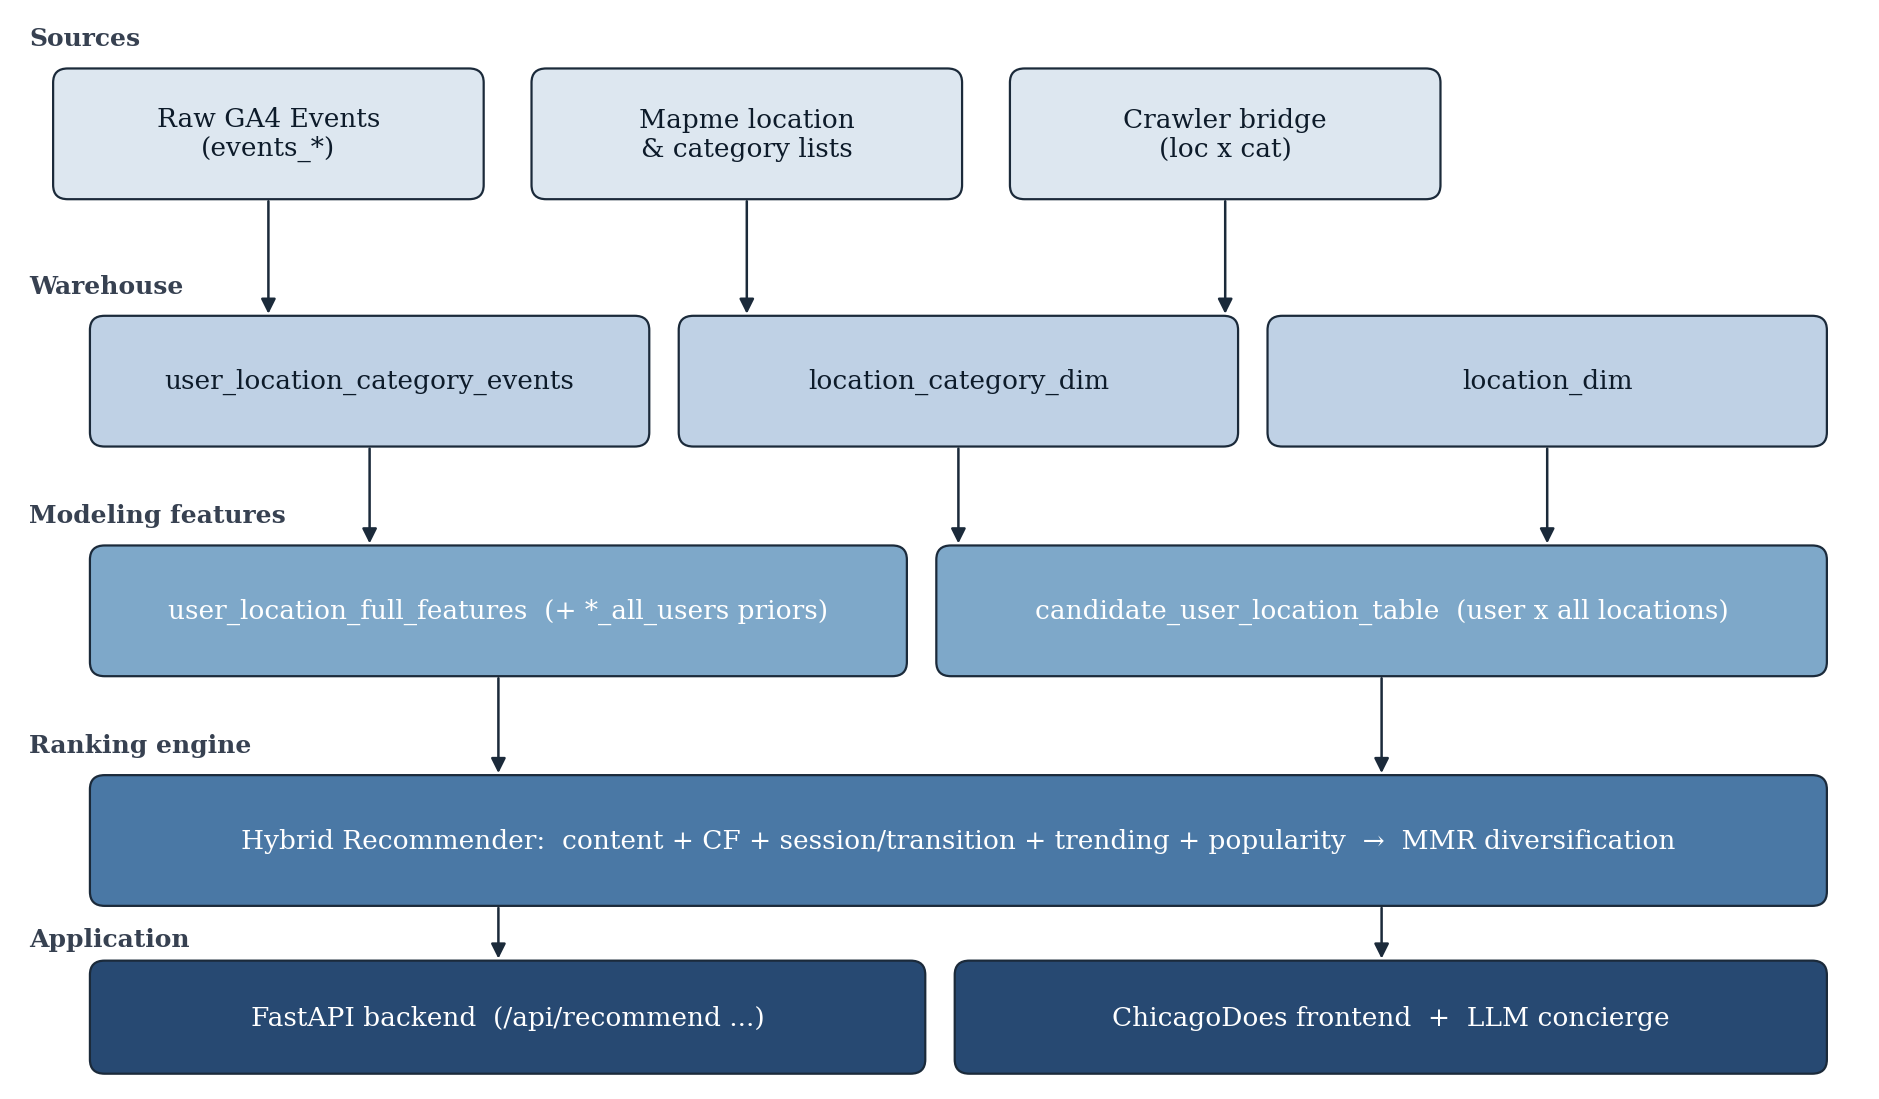
\includegraphics[width=\linewidth]{architecture.png}
\end{figure}

\subsection{Feature Engineering}\label{sec:fe}

Raw GA4 events pass through an engagement-quality filter
(\code{backend/engagement.py}). Events are classified as strong
(\code{map-user-action}, \code{detail\_cta}), weak (\code{page\_view}),
navigation-only (\code{map-search}, \code{session\_start}), or noise
(\code{scroll}). Strong actions are accepted unconditionally; weak
actions require engagement time of at least 1000~ms; navigation-only
and noise events are rejected. Three preset policies
(\code{permissive}, \code{balanced}, \code{strict}) trade off signal
coverage for noise, with \code{balanced} as the production default.
Qualified events are aggregated to the (user, location) grain to
produce \code{user\_location\_full\_features}. For each pair the
warehouse stores total interaction count, event-type-weighted
interaction score, engagement time, distinct sessions, and effective
scores. In parallel, location-level \code{*\_all\_users} aggregates
(distinct users engaged, total interactions, distinct sessions,
average engagement time) are computed user-anonymously and serve as
leakage-safe priors.

Each location is represented as a TF--IDF vector over its category
tokens (\code{recommender.py}). The vectorizer uses L2-normalized
output with a custom token pattern that preserves multi-word
categories such as \code{HOT SPOTS} as a single token. Each location
additionally has two scalar priors (\code{popularity\_norm},
\code{engagement\_norm}) and two binary flags
(\code{is\_hot\_spot\_location}, \code{is\_favorite\_location}). The
location index is built once at application startup and reused for
every recommendation request. Users are represented in two
complementary spaces. The behavioral profile is a weighted average of
the TF--IDF vectors of locations the user interacted with, weighted
by \code{profile\_weight} (derived from interaction score and
engagement). The form-based pseudo-profile is constructed from the
onboarding form (interests, traveler type, vibe, optional free text),
each mapped into category weights via lookup tables
(\code{VIBE\_TO\_CATEGORIES}, \code{TRAVELER\_TO\_CATEGORIES},
\code{FREE\_TEXT\_KEYWORD\_HINTS}) and projected into the same
TF--IDF space. The two profiles are blended at the vector level when
both exist:
\begin{equation}
  \bm{u} = \alpha\,\bm{u}_\text{beh} + (1 - \alpha)\,\bm{u}_\text{form},
  \quad \alpha = 0.6.
  \label{eq:blend}
\end{equation}
One or the other vector is used when only one signal is available.
The dependent quantity that drives ranking is the implicit-feedback
positive: a qualified user--location interaction. Independent
variables are listed in Table~\ref{tab:variables}.

\subsection{Modeling Framework}\label{sec:hybrid}

The recommender implements the weighted-hybrid pattern (Burke, 2002):
each location receives a final score that is a linear combination of
six normalized component scores plus two small categorical boosts.

\subsubsection*{Content Similarity}
Given user profile $\bm{u}$ and location matrix $\bm{L}$ (TF--IDF,
$N \times V$, row-L2-normalized),
\begin{equation}
  s_\text{sim}(i) = \cos(\bm{u}, \bm{L}_i) = \bm{u}^\top \bm{L}_i.
\end{equation}
This term captures categorical fingerprint match between user and
location and is the dominant signal for cold-start visitors whose
only input is the onboarding form.

\subsubsection*{Popularity Prior}
$s_\text{pop}(i) = \texttt{popularity\_norm}(i)$, computed from
\code{*\_all\_users} distinct-user counts and rescaled into $[0, 1]$.
By construction $s_\text{pop}$ does not depend on the current user's
interaction history, making it a leakage-safe prior that prevents
cold-start ranking from being dominated by obscure, low-volume
locations.

\subsubsection*{Item--Item Collaborative Filtering}
Item co-occurrence at the user grain is computed via sparse Jaccard
similarity (\code{collab.py}, \code{ItemCoVisitation}):
\begin{equation}
  J(a, b) = \frac{|U_a \cap U_b|}{|U_a \cup U_b|},
\end{equation}
where $U_x$ is the set of users who engaged with location $x$. At
inference time, the score for candidate $i$ is the mean Jaccard
similarity between $i$ and the user's seed set (their qualified
interactions for returning users, or archetype-popular locations for
cold-start users), min--max normalized to $[0, 1]$.

\subsubsection*{User--User k-Nearest-Neighbor}
User similarity (\code{collab.py}, \code{UserNeighbors}) operates on
L2-normalized category-share vectors: for user $u$ and category $c$,
\[
  \bm{x}_u[c] = \frac{\sum_{\ell \in \mathcal{L}_c} w_{u,\ell}}{\lVert \bm{w}_u \rVert_2},
\]
where $w_{u,\ell}$ is the user's interaction score with location
$\ell$ and $\mathcal{L}_c$ is the set of locations in category $c$.
The top $k = 5$ neighbors of a returning user are identified by
cosine similarity, and the score for candidate $i$ is the average
interaction score that those neighbors recorded on $i$. The term is
zero for cold-start users.

\subsubsection*{Event-Time Trending}
The module \code{trends.py} splits the observation window at the
median timestamp and computes, per location,
\begin{equation}
  \text{trending}_\text{raw}(i) =
  \frac{\text{recent\_weight}(i) + 1}
       {\text{early\_weight}(i) + 1},
\end{equation}
where weight is the sum of \code{interaction\_weight} of events on
$i$ in that half-window. Ratios are min--max normalized to $[0, 1]$.
Locations with fewer than three qualifying events receive a trending
score of zero, preventing low-volume noise.

\subsubsection*{Session Co-Visitation and Transition Graph}
Two additional behavioral signals are derived from raw event sequences
(\code{behavior.py}). Session co-visitation builds a sparse Jaccard
matrix at the session grain rather than the user grain: two locations
that co-occur in many sessions receive high similarity even if no
single user spans both across separate sessions. The transition graph
estimates $P(\text{next}=j \mid \text{previous}=i)$ from the
\code{previous\_location\_id} field GA4 emits on each location view.
The two raw-event signals are blended internally with weights $0.6$
(session-Jaccard) and $0.4$ (transition):
\begin{equation}
  s_\text{sess}(i) = 0.6\,\hat{s}_\text{jacc}(i) + 0.4\,\hat{s}_\text{trans}(i),
\end{equation}
where $\hat{\cdot}$ denotes min--max-normalized component scores.

\subsubsection*{Final Score Blend}
The final score is a weighted sum of the six normalized component
scores plus two small additive boosts for hot-spot and favorite
flags:
\begin{align}
  S(i) =\; & w_\text{sim}\,s_\text{sim}(i)
           + w_\text{pop}\,s_\text{pop}(i)
           + w_\text{item}\,s_\text{item}(i) \nonumber\\
           & + w_\text{user}\,s_\text{user}(i)
           + w_\text{trend}\,s_\text{trend}(i)
           + w_\text{sess}\,s_\text{sess}(i) \nonumber\\
           & + b_\text{hot}\,\mathbb{1}[\text{hot}]
           + b_\text{fav}\,\mathbb{1}[\text{fav}].
  \label{eq:final}
\end{align}
Two weight vectors are used depending on user regime, initially
calibrated by signal availability (Table~\ref{tab:weights} and
Figure~\ref{fig:blend}); the returning-user schedule was subsequently
re-tuned through the cross-validated weight search described in
the Evaluation Methodology subsection, with the tuned values reported
in the Findings section. The categorical boosts are
$b_\text{hot} = 0.12$ and $b_\text{fav} = 0.03$. Hot-spot locations
correspond to ChicagoDoes' paid advertiser placements; at the
sponsor's request $b_\text{hot}$ was raised from an initial $0.05$ to
$0.12$, which increases the hot-spot share of top-10 recommendations
from roughly 43\% to 52\% across demo personas while leaving offline
NDCG@10 unchanged within sampling noise, and the value is exposed as a
deployment-time environment variable so the business can retune it
without a code change. After scoring, the
candidate set is filtered to respect interest and avoid-category
constraints, and already-interacted locations are excluded for
returning users.

\begin{table}[H]
\centering
\caption[Component weights in the final score blend by user regime]{Component weights in the final score blend by user regime (\code{WEIGHTS\_NEW} vs.\ \code{WEIGHTS\_RETURNING} in \code{recommender.py})}
\label{tab:weights}
\small
\rowcolors{2}{tableheader!40}{white}
\begin{tabularx}{\linewidth}{Xrrrrrr}
\toprule
\thead[l]{Regime} & \thead[r]{$w_\text{sim}$} &
\thead[r]{$w_\text{pop}$} & \thead[r]{$w_\text{item}$} &
\thead[r]{$w_\text{user}$} & \thead[r]{$w_\text{trend}$} &
\thead[r]{$w_\text{sess}$} \\
\midrule
New visitor      & 0.40 & 0.20 & 0.10 & 0.00 & 0.10 & 0.20 \\
Returning user   & 0.22 & 0.15 & 0.18 & 0.20 & 0.05 & 0.20 \\
\bottomrule
\end{tabularx}
\end{table}

\begin{figure}[H]
  \centering
  \caption{Score-blend weights by user regime. For new visitors, content and session signals dominate; for returning users, user--user kNN contributes a fifth of the blend, replacing part of the content weight}
  \label{fig:blend}
  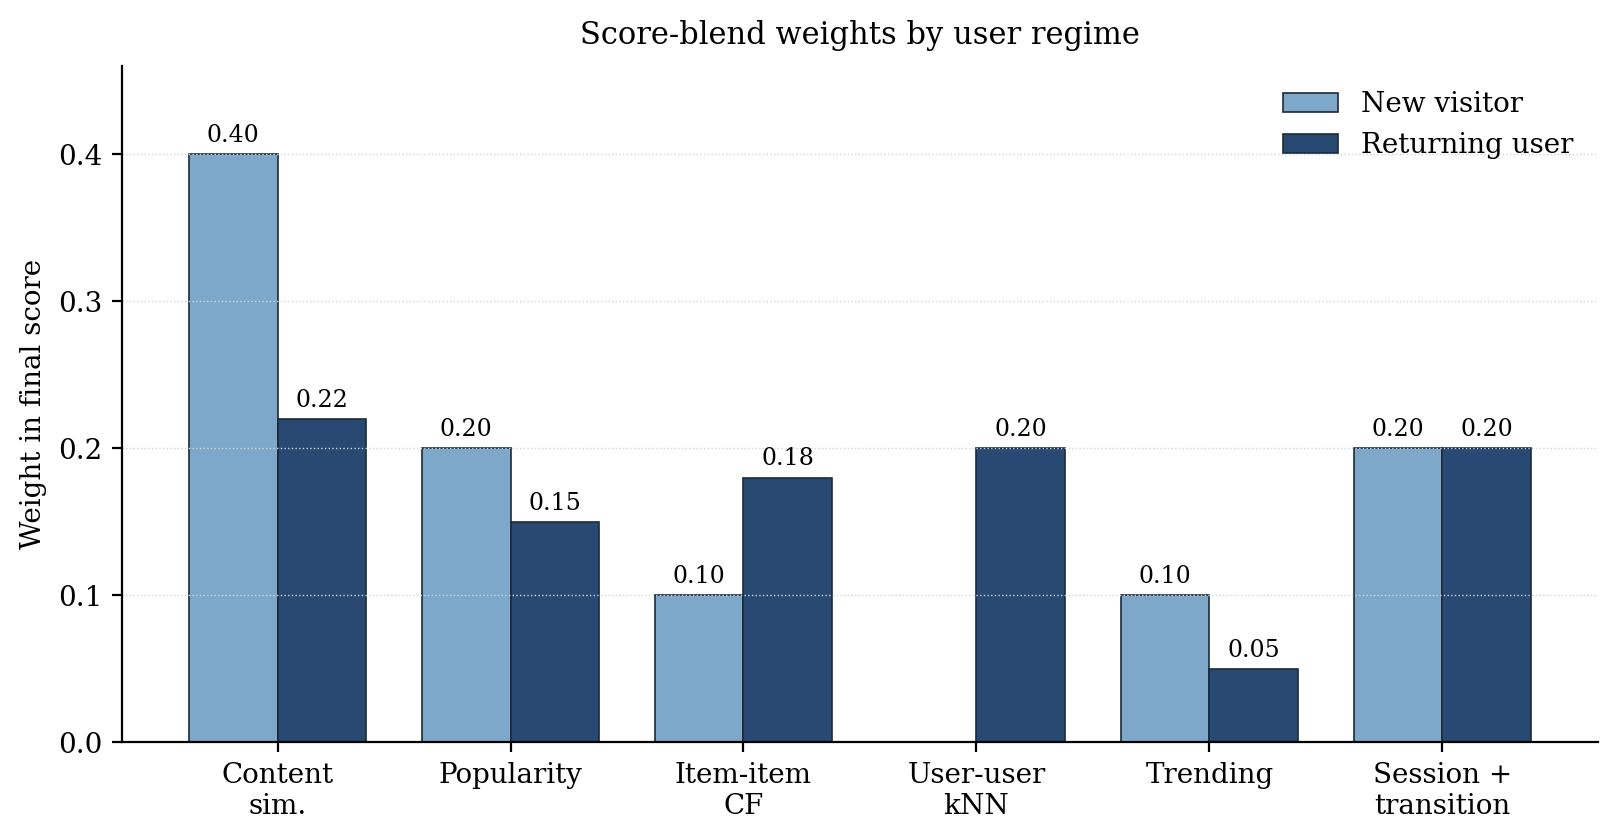
\includegraphics[width=0.9\linewidth]{score_blend.png}
\end{figure}

\subsection{Cold-Start Handling and User Archetypes}\label{sec:cold}

Cold-start was the central operational challenge for ChicagoDoes given
the high proportion of single-session anonymous visitors. The system
handles it through two complementary mechanisms. First, the
onboarding form provides explicit preference signals (interests,
traveler type, vibe, optional free text) that are mapped through
lookup tables into category weights and projected into the same
TF--IDF space as locations, producing an immediately usable
pseudo-profile. Second, behavioral archetypes are computed by
$K$-Means clustering (\code{segments.py}) over category-share vectors
of returning users with non-trivial histories. The number of clusters
is set to $k = 6$, which empirically gives meaningful separation for
a user base of several hundred users without splintering. Each
cluster is given a human-readable archetype label by looking up the
dominant category in its centroid (for example, Outdoor Wanderer,
Cultural Enthusiast, Nightlife Seeker, Foodie Wanderer, Sightseeing
Explorer). A cold-start user's form vector is projected into the same
space and assigned to the nearest centroid, providing both a
displayable persona and a seed set of locations (the most popular
locations among users in that cluster). The seed set powers the
item--item collaborative term for cold-start visitors who would
otherwise have no anchor to compute against.

\subsection{Diversity Re-Ranking}\label{sec:mmr}

Pointwise ranking by $S(i)$ produces homogeneous lists when a category
aligns strongly with the user's profile (for example, a foodie user
ending up with ten consecutive restaurants). Maximal Marginal
Relevance (Carbonell \& Goldstein, 1998) is applied as
post-processing. Given a candidate pool of the top 60 candidates by
$S$, MMR iteratively selects the next item to maximize
\begin{equation}
  \text{MMR}(i) = \lambda \cdot S(i)
                - (1 - \lambda)\,\max_{j \in \mathcal{S}}
                  \cos(\bm{L}_i, \bm{L}_j),
  \label{eq:mmr}
\end{equation}
where $\mathcal{S}$ is the set of already-selected items. The trade
parameter is $\lambda = 0.7$ (70~percent relevance, 30~percent
diversity); a schematic is shown in Figure~\ref{fig:mmr}.

\begin{figure}[H]
  \centering
  \caption{MMR re-ranking selects from the top-60 candidates by raw score and iteratively trades relevance against distance from already-picked items}
  \label{fig:mmr}
  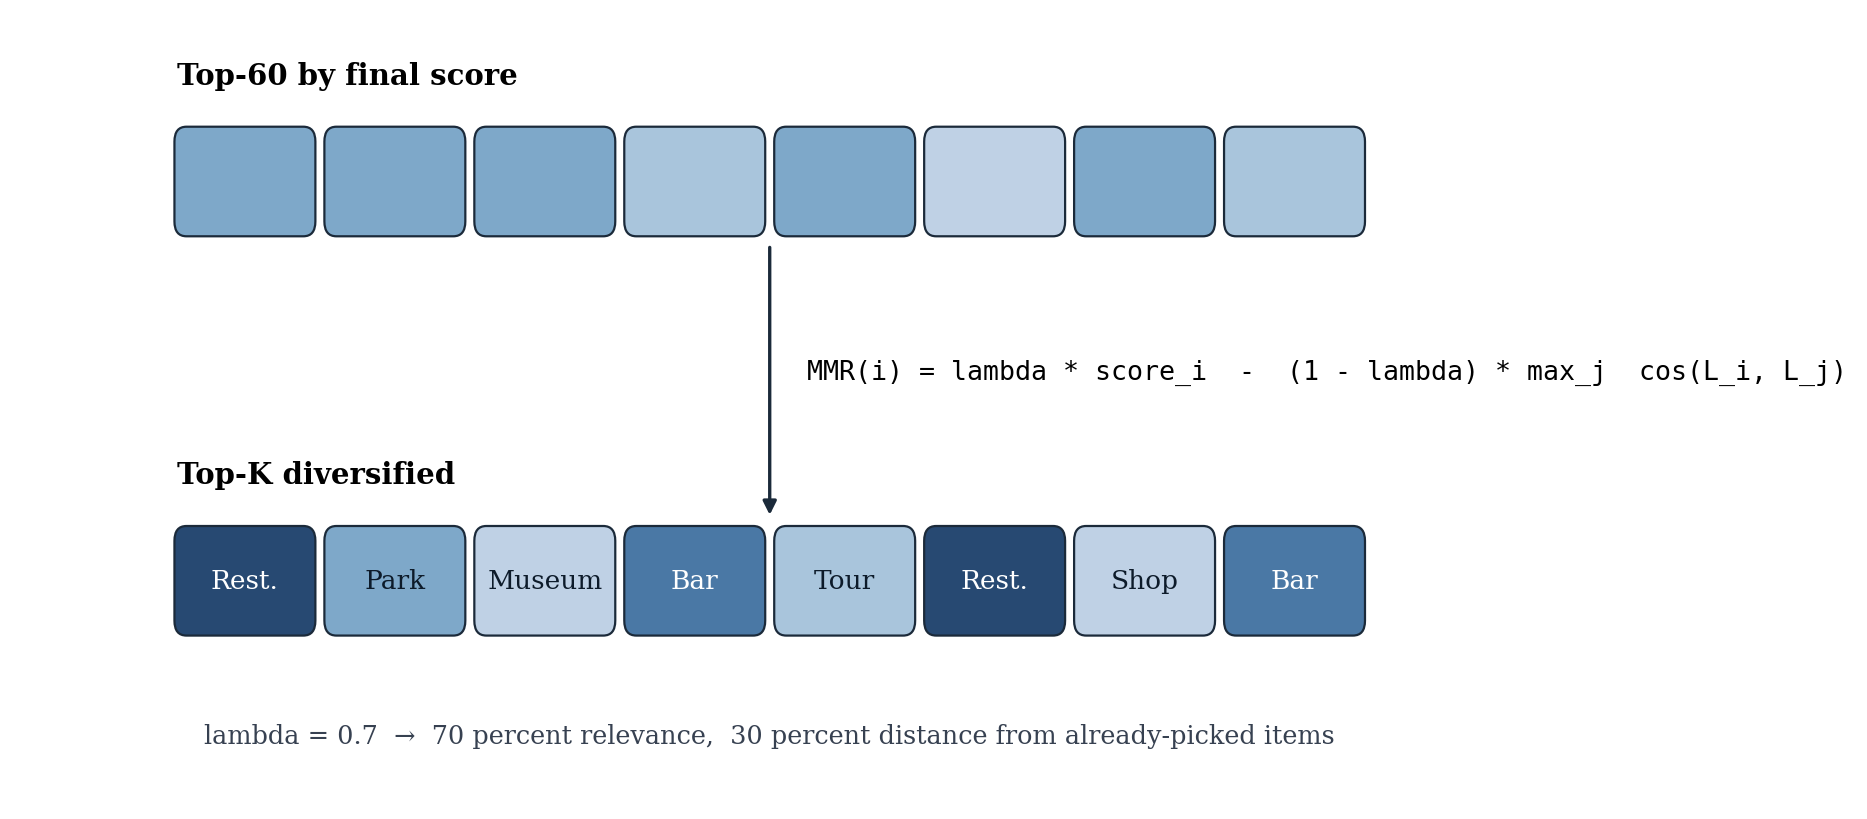
\includegraphics[width=0.9\linewidth]{mmr_diagram.png}
\end{figure}

\subsection{LLM Concierge and Itinerary Layer}\label{sec:llm}

An optional LLM concierge layer (\code{llm\_service.py},
\code{itinerary\_llm.py}) provides natural-language outputs for
explanation and itinerary planning. The strict product rule is that
the LLM may only schedule or describe locations already in the
current recommendation pool: it is given a JSON list of
\code{location\_id} values drawn from the top-$K$ and is prompted to
produce a multi-day itinerary, a per-card ``Why this?'' explanation,
or a ``More info'' concierge blurb. A natural-language refinement
endpoint (\code{/api/refine}) additionally lets the visitor adjust an
existing itinerary with free-text requests, such as swapping a stop
or slowing a day's pace, while remaining restricted to the same
deterministic pool. If the LLM is unreachable or
returns invalid JSON, deterministic templates and a fallback
scheduler ensure the experience degrades gracefully. This decoupling
preserves the ranking guarantees of the deterministic recommender
while still allowing user-facing copy to feel natural and varied.

\subsection{Interface Delivery and Media Enrichment}\label{sec:media}

The user-facing application was redesigned around a media-rich card
interface showing, for each recommendation, a venue photograph or
video, category tags, an evidence block, and a one-line specialty
blurb. Venue media were resolved offline through Firecrawl, a
managed web-crawling and scraping service
(\code{scripts/build\_location\_cards.py},
\code{backend/chicagodoes\_media.py}): for every catalog location
the pipeline scrapes photographs and videos from the venue's
ChicagoDoes listing and gallery pages, falls back to the venue's
official website only when the listing has no media, and stores
localized copies so no crawling occurs at request time. The same
pipeline resolves each venue's ChicagoDoes listing URL, and both the
card photograph and the card title link to that listing, routing
recommender-driven engagement back onto the client's platform. A
companion script repairs defaulted map coordinates through Firecrawl
search and geocoding, and duplicate suppression by canonical place
name prevents the same venue from appearing twice in a list.

\subsection{Feedback-Loop Prevention}\label{sec:guard}

Because the recommender operates on the same GA4 telemetry that its
own interface generates, outbound clicks from recommendation cards
into ChicagoDoes could create a self-reinforcing feedback loop:
recommended venues would accumulate engagement events, appear
organically more popular in the next warehouse refresh, and be
recommended even more often. Three complementary mechanisms were
implemented to break this loop. First, every outbound link is tagged
at click time with attribution parameters
(\code{utm\_source=ateema\_recommender}, \code{rec\_source},
\code{rec\_surface}, \code{rec\_rank}, \code{rec\_location\_id}) so
that downstream GA4 and BigQuery training pipelines can identify and
exclude, rather than ingest, recommender-origin sessions when
rebuilding popularity and engagement aggregates. Second,
recommender-origin clicks are logged separately through a dedicated
endpoint (\code{/api/outbound/click}) to an append-only local store
(\code{data/outbound\_clicks.jsonl}); they are retained as an
attribution and control signal but are never treated as positive
engagement labels. Third, a runtime guard
(\code{ContentRecommender.\_build\_feedback\_penalty()}) subtracts a
small penalty proportional to each location's normalized volume of
recent recommender-origin clicks from its final score, with a default
strength of $0.08$ over a 30-day window, damping any residual
self-reinforcement between warehouse refreshes. The guard is
configurable through environment variables and its status is exposed
by the health endpoint.

\subsection{Evaluation Methodology}\label{sec:eval}

Offline ranking evaluation was implemented in
\code{backend/evaluation.py} and \code{backend/evaluation\_runner.py}
following the conventions of the implicit-feedback literature (Hu
et~al., 2008; Cremonesi et~al., 2010). Qualified user--location
interactions were partitioned per user with a leave-last-one temporal
split: for each returning user with sufficient history, the most
recent qualified interaction was held out as the test item, and all
warehouse-side aggregates, including popularity priors, collaborative
matrices, trending scores, and behavioral profiles, were rebuilt
strictly from training-period events so that no held-out interaction
could leak into the features that score it. A temporal split was
preferred over random splitting because the trending and
session-co-visitation signals are time-aware. Held-out items were
scored with Precision@K, Recall@K, Hit Rate@K, NDCG@K, and Mean
Average Precision at $K \in \{5, 10, 20\}$, with NDCG@10 as the
primary tuning metric because it rewards placing the held-out item
near the top of the list, which matches the shallow exploration depth
observed in the Descriptive Analysis subsection. The hybrid ranker was
benchmarked against a global-popularity ranker, a content-only
TF--IDF ranker, a collaborative-only ranker, and the hybrid without
MMR, isolating both the value of hybridization and the accuracy cost
of diversification. Score-blend weights were then tuned by a
randomized search over more than 4{,}000 weight configurations on the
simplex, and the surviving configurations were validated with
five-fold cross-validation over users
(\code{backend/weight\_search\_cv.py}): within each fold the best
configuration was selected in-sample and scored on the held-out fold,
and a robust configuration was formed by averaging the per-fold
winners. The gap between in-sample and held-out scores was tracked as
an overfitting diagnostic. All evaluation, search, and
cross-validation runs were logged to MLflow
(\code{backend/mlflow\_track.py}) for reproducibility and comparison.
The existing \code{scripts/evaluate\_engagement\_impact.py} script
complements the harness by comparing recommendations with and without
engagement filtering. The harness is designed to extend beyond
ranking accuracy in subsequent evaluation rounds: catalog coverage
(the fraction of the catalog ever appearing in any user's top-$K$),
novelty (average inverse popularity), and category entropy of the
recommended lists; a random-within-interest baseline; per-signal
ablation studies quantifying each component's marginal contribution;
sensitivity of results to the engagement-filter policy
(\code{permissive} versus \code{balanced} versus \code{strict}); and
bootstrap stability of the $K$-Means archetypes are scoped for the
next round as interaction volume grows. Once the system is deployed
behind a feature
flag, an online A/B test will compare the personalized experience
against the current default (no personalization). Primary online
metrics will be locations viewed per session, click-through rate on
recommended locations, session duration,
\code{section-details-call-to-action} conversions, and return-visit
rate among identified users; secondary metrics will track
partner-side impressions and CTA clicks attributed to paying venues.

% =====================================================================
\section{Findings}\label{sec:findings}

Findings are reported across four groups: descriptive findings drawn
directly from GA4 telemetry, design-validation findings derived from
warehouse construction and the modeling pipeline, quantitative
results from the offline ranking evaluation and weight search
described in the Evaluation Methodology subsection, and qualitative findings observed in
the live application.

\subsection{Engagement Patterns Are Heavy-Tailed and Repeat-Driven}

Across the observation window, total location clicks were dominated
by a small head of venues. Garrett Popcorn Shops received 31 total
clicks from 17 unique users, the highest on both axes
(Figure~\ref{fig:listings}). The second-ranked listing by total
clicks, Roll Up, accumulated those clicks from only two unique users,
yielding a click-to-user ratio more than ten times the head of the
distribution. The discrepancy demonstrated empirically that ranking
by raw clicks would over-promote repeat-visit listings that lack
broad appeal. This finding motivated the recommender's popularity
prior to be computed from \code{popularity\_norm} (distinct users
engaged) rather than from raw event counts, eliminating the bias.

\subsection{Strong-Action Events Are a Small Fraction of Map Activity}

Of the 403 users who loaded the map (Figure~\ref{fig:funnel}), 62
(15 percent) clicked an individual map marker. At the same time, 188
users reached the listing detail page via the
\code{section-details-call-to-action} event, three times the
marker-click count. This funnel diverged from the assumption that
detail-page reach implies a prior marker click and demonstrated that
many users discover listings through list browsing and category
filtering rather than direct map interaction. The recommender was
therefore designed to treat \code{map-marker-click} and
\code{section-details-call-to-action} symmetrically as
\code{STRONG\_ACTIONS} (\code{backend/engagement.py}), preventing
either path from being inadvertently down-weighted.

\subsection{Exploration Depth Is Low; Front-Loading Matters}

Over half of users clicked only one or two listings per session
(Figure~\ref{fig:depth}). The implication is that, in practice, the
recommender has at most two opportunities to surface the right
content per user. This evidence reinforced the choice to apply
diversity re-ranking via MMR with a 30~percent diversity weight
(see Diversity Re-Ranking): when users sample only the very top of the list,
homogeneous results disproportionately damage the user experience.

\subsection{Entry-Point Patterns Confirm Multi-Intent Visitors}

Entry-point analysis (Figure~\ref{fig:entry}) identified three
distinct first-click clusters around food and snacks (Garrett Popcorn
Shops, 9 first-click users), accommodation (The Evie hotel), and
landmarks (Navy Pier). Heterogeneity of first-click intent provided
direct empirical justification for the behavioral archetype system
(see Cold-Start Handling and User Archetypes): a single global popularity head would mask these
sub-populations, whereas $K$-Means segmentation over category-share
vectors yields six interpretable archetypes (Foodie Wanderer,
Sightseeing Explorer, Cultural Enthusiast, Nightlife Seeker, Outdoor
Wanderer, Comfort Traveler) whose dominant categories align with the
observed entry-point spectrum.

\subsection{Temporal Activity Validates Time-Split Trending}

Activity was strongly concentrated on Saturday between 11~a.m. and
3~p.m., with secondary weekday early-afternoon spikes
(Figure~\ref{fig:temporal}). Activity between 3 and 9~a.m. was
negligible across all days. The presence of distinct active and
inactive windows validated the median-timestamp split used by the
event-time trending signal in \code{backend/trends.py}: the split
point falls within an active period and produces meaningfully
populated halves for the recent-to-early ratio.

\subsection{Layered Warehouse Successfully Decouples Priors from Per-User Features}

The warehouse implementation produced the seven-layer pipeline
documented in Table~\ref{tab:warehouse}, terminating in
\code{user\_location\_full\_features} (per-pair behavior plus
\code{*\_all\_users} priors) and \code{candidate\_user\_location\_table}
(the full user-by-location candidate set). The decoupling between
\code{*\_all\_users} priors and per-user features is the operational
realization of the leakage-safe design: predictive features in the
ranking blend (popularity, engagement, trending) read only from the
priors layer, while per-user counts are isolated to behavioral profile
construction. A spot check across sample users confirmed that
swapping in or out a user's interaction record does not alter the
priors that score their candidates.

\subsection{Hybrid Score Blend Yields Differentiated Top-K Lists Across User Regimes}

Inspection of top-$K$ outputs across new-visitor and returning-user
weight schedules (Table~\ref{tab:weights}) confirmed that the two
regimes produce qualitatively different rankings on shared inputs.
For cold-start users, the new-visitor schedule (with content weight
0.40 and session weight 0.20) recovered the form-derived category
fingerprint; for returning users, the same locations were re-ranked
to elevate items reached by user--user $k$-NN ($w_\text{user} = 0.20$)
and to suppress already-interacted locations via the
exclusion filter. The presence of distinct, regime-dependent rankings
on identical candidate pools demonstrated that the weight schedules
behave as intended.

\subsection{Offline Evaluation: Content and Popularity Signals Dominate at Current Data Scale}

The offline harness evaluated 120 returning users under the
leave-last-one temporal split over the GA4 window from April~27 to
May~17, 2026 (approximately three weeks and 12{,}000 events).
Table~\ref{tab:offline} reports the ranking metrics at $K = 10$. The
content-only TF--IDF baseline achieved the highest held-out accuracy
(NDCG@10 of 0.223), outperforming the full hybrid under its original
returning-user weights both without MMR (0.201) and with MMR (0.164),
while the popularity baseline trailed all learned variants (0.121).
The original hybrid weights therefore under-delivered relative to the
strongest single signal: at the current data scale, dominated by
single-session users, the collaborative and session matrices are too
sparse to carry the 0.58 combined weight assigned to them in the
original returning-user schedule, and their noise diluted the
content and popularity signals.

\begin{table}[H]
\centering
\caption[Offline ranking metrics at $K=10$ for the hybrid and baselines]{Offline ranking metrics at $K = 10$ on 120 held-out returning users (leave-last-one temporal split, original weight schedules)}
\label{tab:offline}
\small
\rowcolors{2}{tableheader!40}{white}
\begin{tabularx}{\linewidth}{Xrrrr}
\toprule
\thead[l]{Ranker} & \thead[r]{P@10} & \thead[r]{HR@10} &
\thead[r]{NDCG@10} & \thead[r]{MAP@10} \\
\midrule
Content-only (TF--IDF)   & 0.038 & 0.383 & 0.223 & 0.174 \\
Hybrid without MMR       & 0.036 & 0.358 & 0.201 & 0.153 \\
Collaborative-only       & 0.029 & 0.292 & 0.169 & 0.131 \\
Hybrid with MMR          & 0.027 & 0.267 & 0.164 & 0.134 \\
Global popularity        & 0.022 & 0.217 & 0.121 & 0.092 \\
\bottomrule
\end{tabularx}
\end{table}

\subsection{Cross-Validated Weight Re-Tuning Improves Held-Out Ranking}

The randomized search over more than 4{,}000 weight configurations,
validated with five-fold cross-validation over users, confirmed that
the under-performance was a weighting problem rather than a design
problem. Within each fold the best configuration was selected on the
in-fold users and then scored on the held-out fold, so every reported
gain reflects users the winning configuration never saw.
Table~\ref{tab:cv} reports the per-fold results. The fold winners
improved held-out NDCG@10 by 20.6 percent on average over the
original returning-user schedule, winning four of five folds; the
single losing fold (fold 2, $-3.4$ percent) reflects the expected
fold-to-fold variance at this sample size rather than a
contradiction. The gap between in-sample and held-out scores stayed
small (mean 0.019), indicating that the search was not simply
memorizing the validation users.

\begin{table}[H]
\centering
\caption[Per-fold cross-validation results for the weight search]{Per-fold cross-validation results: held-out NDCG@10 of the in-fold winning configuration versus the original returning-user weights (24 users per fold)}
\label{tab:cv}
\small
\rowcolors{2}{tableheader!40}{white}
\begin{tabularx}{\linewidth}{Xrrrr}
\toprule
\thead[l]{Fold} & \thead[r]{In-sample} & \thead[r]{Held-out} &
\thead[r]{Held-out (orig.)} & \thead[r]{Gain} \\
\midrule
1 & 0.260 & 0.225 & 0.191 & $+17.8\%$ \\
2 & 0.259 & 0.223 & 0.231 & $-3.4\%$  \\
3 & 0.257 & 0.243 & 0.199 & $+22.4\%$ \\
4 & 0.257 & 0.263 & 0.198 & $+32.6\%$ \\
5 & 0.261 & 0.248 & 0.185 & $+33.5\%$ \\
\bottomrule
\end{tabularx}
\end{table}

The direction of the re-weighting, shown in Table~\ref{tab:tuned},
is explainable signal by signal from the data conditions documented
in the Data section. The popularity weight tripled (0.15 to 0.45)
because the popularity prior is the only behavioral signal that is
dense: it is defined for every candidate location, it is computed
from distinct users rather than raw clicks, and it is leakage-safe
by construction, which makes it the most reliable ranking evidence
at a scale of roughly three weeks of events. Content similarity rose
(0.22 to 0.30) for a similar reason: the TF--IDF category vector
exists for every location regardless of interaction volume, so the
content term generalizes to the long tail of rarely visited venues.
The item-collaborative and session weights collapsed (0.18 to 0.04
and 0.20 to 0.03) because their underlying co-occurrence matrices
are nearly empty when most visitors appear in a single session and
click one or two listings: with so few co-visits, a large weight on
these terms does not add signal but amplifies noise, over-promoting
whichever locations happen to share a handful of sessions. In
effect, the original schedule had allocated a combined 0.58 of the
blend to co-occurrence signals sized for a denser interaction log
than the platform has yet accumulated. The user--user kNN weight
declined more moderately (0.20 to 0.14) but was the least stable
component across folds (fold-to-fold standard deviation of
$\pm 0.20$ in Table~\ref{tab:tuned}), indicating that neighbor
quality depends strongly on which users land in the training split;
the trending weight was essentially unchanged.

\begin{table}[H]
\centering
\caption[Original versus CV-validated returning-user weights]{Original versus cross-validation-validated component weights for the returning-user path, with fold-to-fold standard deviation of the validated values}
\label{tab:tuned}
\small
\rowcolors{2}{tableheader!40}{white}
\begin{tabularx}{\linewidth}{Xrrr}
\toprule
\thead[l]{Component} & \thead[r]{Original} & \thead[r]{CV-validated} & \thead[r]{Fold s.d.} \\
\midrule
Content similarity $w_\text{sim}$      & 0.22 & 0.30 & $\pm 0.09$ \\
Popularity $w_\text{pop}$              & 0.15 & 0.45 & $\pm 0.14$ \\
Item--item CF $w_\text{item}$          & 0.18 & 0.04 & $\pm 0.03$ \\
User--user kNN $w_\text{user}$         & 0.20 & 0.14 & $\pm 0.20$ \\
Trending $w_\text{trend}$              & 0.05 & 0.04 & $\pm 0.04$ \\
Session/transition $w_\text{sess}$     & 0.20 & 0.03 & $\pm 0.02$ \\
\bottomrule
\end{tabularx}
\end{table}

The retained configuration is the average of the five fold winners
rather than the single best configuration found anywhere in the
search. With 120 evaluable users, the globally best configuration is
partly an artifact of which held-out interactions it happened to
fit, so averaging trades a small amount of in-sample score for
stability. The averaged configuration still outperformed the
original schedule on held-out users (NDCG@20 of 0.256 versus 0.248,
a 3.2 percent gain, winning three of five folds, with an
in-sample-to-held-out gap of 0.025) and was retained as the
validated weight set for the returning-user path
(\code{data/robust\_weights.json}). Three caveats bound this result.
Confidence intervals between neighboring configurations overlap at
this sample size, so the direction of the re-weighting is robust but
the exact optimal values are not. The protocol covers returning
users only, so the new-visitor schedule remains untested. And the
tuned weights are a snapshot of a three-week log: as multi-session
histories accumulate, the collaborative and session terms are
expected to earn weight back, which is why the search and
cross-validation are scripted and MLflow-tracked so the tuning can
be repeated cheaply on each warehouse refresh.

\subsection{MMR Diversification Visibly Restructures the Top-K}

When MMR was switched on with $\lambda = 0.7$, the top-$K$ lists
produced for foodie-leaning and culture-leaning profiles consistently
re-shuffled out one or two near-duplicate same-category venues per
list (for example, two adjacent restaurants from the same cuisine
family) in favor of items from the next-closest categories. The
re-shuffling occurred without removing the user's primary category
from the list and without dropping the relevance-leader. The offline
harness quantified the trade-off: under the tuned weights, enabling
MMR reduced held-out NDCG@10 from 0.256 to 0.240 (a 6~percent
accuracy cost) while raising mean intra-list diversity from 0.277 to
0.604, an increase of 118~percent. Given the shallow exploration
depth documented in the Descriptive Analysis subsection, the diversity gain was
judged to outweigh the accuracy cost, and MMR was retained in
production.

\subsection{Application-Level Findings}

The deterministic recommendation pool was wrapped by a FastAPI
backend and a redesigned JavaScript frontend that exposes
recommendation cards with evidence blocks (distinct users engaged,
total interactions, average dwell time, trending flag). The
Firecrawl media pipeline resolved verified photographs or videos for
the catalog locations surfaced on recommendation cards, and every
card links to the venue's ChicagoDoes listing page. The
feedback-loop guard operated as designed in spot checks: outbound
clicks arrived at ChicagoDoes carrying the
\code{ateema\_recommender} attribution parameters, were logged to
the separate outbound-click store rather than the engagement
pipeline, and the health endpoint reported the guard active with its
default strength. The LLM concierge endpoint
(\code{/api/explain}, \code{/api/itinerary}) was constrained to the
deterministic top-$K$ pool; in spot-check trials it produced
fluent ``Why this?'' rationales and multi-day itineraries that never
referenced a location outside the supplied list, demonstrating that
the LLM serves as a presentation layer rather than as an unbounded
candidate generator. Fallback templates and the deterministic
scheduler engaged correctly when the LLM endpoint was disabled,
confirming graceful degradation. The application was containerized
and deployed as a public website: a Docker image serves the FastAPI
application on Google Cloud Run with the verified card media bundled
into the image so no crawling occurs in production, and a Render
blueprint (\code{render.yaml}) provides a free-tier deployment
alternative. When BigQuery credentials are absent, the deployment
automatically falls back to a bundled demonstration dataset, so the
public site remains fully functional without live warehouse access.

% =====================================================================
\section{Discussion}\label{sec:discussion}

Several themes emerge from design and implementation. First, the
choice of a hybrid weighted recommender rather than a single
matrix-factorization model is well-justified by the data: interaction
sparsity is high, the user base is dominated by single-session
anonymous visitors, and explicit feedback is absent. Under these
conditions, content-based signals provide essential coverage that
pure matrix factorization could not, and the additional collaborative
and session-level terms provide refinement once interactions
accumulate. The descriptive findings mirror
the conditions that the recommendation literature identifies as
favorable for hybridization (Burke, 2002; \c{C}ano \& Morisio, 2017).

Second, leakage discipline was a design choice with practical
consequences. By restricting predictive features to user-anonymous
priors and behavioral vectors that summarize prior interactions
without copying them as labels, the recommender remains honest under
offline evaluation: a user's held-out interactions cannot leak into
the features that score them. The separation between
\code{*\_all\_users} priors (used as priors) and per-user interaction
counts (used only to construct the behavioral profile vector) is the
operational enforcement of that boundary.

Third, the offline evaluation sharpened, rather than merely
confirmed, the design. The finding that a content-only ranker beat
the original hybrid weighting (Table~\ref{tab:offline}) does not
argue against hybridization; it shows that the hand-set
returning-user schedule over-weighted collaborative and session
signals that a three-week, mostly single-session window cannot yet
support. Once the weights were re-tuned under cross-validation, the
hybrid recovered and exceeded the content-only baseline on held-out
users, and the tuned direction, heavier content and popularity with
near-zero session and item-collaborative weight, is exactly what the
sparsity conditions predict. The hyper-parameters that were
placeholders at design time are now empirically grounded: the
returning-user weight schedule carries a cross-validated
configuration, and the MMR $\lambda$ in Equation~\ref{eq:mmr} was
retained after its accuracy-for-diversity trade-off was measured
rather than assumed. Two evaluation caveats bound these claims: with
120 evaluable users the confidence intervals of neighboring
configurations overlap, and the returning-user path that the tuning
targets is dormant in the live site until visitors are linked to
persistent identities, so all live traffic is currently scored with
the new-visitor schedule. Online validation therefore remains the
largest open question.

A further design theme concerns data integrity. A recommender that
sits on top of the telemetry it influences will, if left unguarded,
gradually contaminate its own training signal, since every
recommended venue accrues clicks that the next model refresh reads
as organic popularity. The three-layer guard described in the methodology,
attribution tagging for warehouse-side exclusion, separate outbound
logging, and a runtime penalty, converts recommender-driven traffic
from a hidden bias into an explicit, controllable signal. This
protects not only the model but also the client's analytics: partner
reporting on ChicagoDoes engagement remains interpretable because
recommender-origin sessions are identifiable.

Fourth, several limitations are intrinsic to the data rather than to
the model. The absence of explicit ratings, the short observation
window, the predominance of single-session users, and the loss of
conversion signal after a user leaves the platform are all properties
of the GA4 export rather than choices in the methodology. The
recommender design is robust to these constraints, but they bound
what any recommender on this data can achieve. The findings reported
in the Findings section should be interpreted within these data
limits and not extrapolated to seasonal regimes, identified-user
populations, or post-visit conversion outcomes that the present GA4
window does not capture.

% =====================================================================
\section{Conclusion}\label{sec:conclusion}

This capstone designed and implemented a personalized
location-recommendation system for ChicagoDoes end-to-end.
Deliverables include a layered BigQuery data warehouse that converts
raw GA4 events into modeling-ready features; a hybrid recommender
blending six complementary scoring signals into a single ranking; a
diversity-aware MMR re-ranker; a $K$-Means-based behavioral archetype
system for cold-start visitors; an offline evaluation harness with
baseline comparison, cross-validated weight search, and MLflow
tracking; a feedback-loop guard that keeps recommender-driven clicks
out of the training signal; and a full-stack web application,
containerized and deployed publicly on Google Cloud Run, that
demonstrates the system live with evidence-backed, media-rich
recommendation cards linking to ChicagoDoes listings and an optional
LLM concierge layer for explanation and itinerary planning. The
descriptive findings established that
ChicagoDoes engagement is heavy-tailed, repeat-driven, and shallow,
and that distinct entry-point intents coexist in the user
population, all of which directly shaped the design of the popularity
prior, the strong-action classification, the behavioral archetypes,
and the diversity re-ranker.

The immediate impact of the system for the client is threefold: it
converts a previously unused GA4 stream into a structured,
queryable warehouse that supports future analytics and recommendation
work; it delivers a deployable personalization layer, validated
offline with an approximately 20~percent held-out NDCG@10 improvement
from cross-validated weight tuning, that can be turned on behind a
feature flag against the current default experience; and it routes
recommender-driven engagement back to ChicagoDoes listings under
explicit attribution, so the personalization layer feeds the client's
platform without distorting its analytics. The work scoped for the
next deployment phase has four strands. Identity linking (for
example, GA4 client ID or QR attribution) will activate the dormant
returning-user path, which already carries its cross-validated weight
configuration, and will extend the evaluation protocol to cold-start
visitors; subsequent offline rounds will add the coverage, novelty,
ablation, and stability analyses scoped in the evaluation
methodology. An online A/B test will quantify the engagement uplift of
the personalized experience against the current default and confirm
partner-side benefits. A retrieval-augmented generation extension
will ground the LLM concierge layer in richer location descriptions
(reviews, photos, structured tags) without permitting hallucinated
content. Usability testing will inform further refinements to the
onboarding form, the evidence block, and the itinerary visualization.
The same methodology is recommended for straightforward extension to
other Ateema city properties beyond Chicago once a comparable GA4
export window is available.

% =====================================================================
\section{References}\label{sec:references}
\begingroup
\singlespacing
\setlength{\parskip}{6pt}
\newcommand{\refitem}{\par\hangindent=0.5in\hangafter=1\noindent}

\refitem
Aggarwal, C.~C. (2016). \textit{Recommender systems: The textbook}. Springer. \url{https://doi.org/10.1007/978-3-319-29659-3}

\refitem
Borr\'{a}s, J., Moreno, A., \& Valls, A. (2014). Intelligent tourism recommender systems: A survey. \textit{Expert Systems with Applications, 41}(16), 7370--7389. \url{https://doi.org/10.1016/j.eswa.2014.06.007}

\refitem
Burke, R. (2002). Hybrid recommender systems: Survey and experiments. \textit{User Modeling and User-Adapted Interaction, 12}(4), 331--370. \url{https://doi.org/10.1023/A:1021240730564}

\refitem
Carbonell, J., \& Goldstein, J. (1998). The use of MMR, diversity-based reranking for reordering documents and producing summaries. In \textit{Proceedings of the 21st annual international ACM SIGIR conference on research and development in information retrieval} (pp.~335--336). ACM. \url{https://doi.org/10.1145/290941.291025}

\refitem
\c{C}ano, E., \& Morisio, M. (2017). Hybrid recommender systems: A systematic literature review. \textit{Intelligent Data Analysis, 21}(6), 1487--1524. \url{https://doi.org/10.3233/IDA-163209}

\refitem
Cremonesi, P., Koren, Y., \& Turrin, R. (2010). Performance of recommender algorithms on top-$N$ recommendation tasks. In \textit{Proceedings of the fourth ACM conference on recommender systems} (pp.~39--46). ACM. \url{https://doi.org/10.1145/1864708.1864721}

\refitem
Gavalas, D., Konstantopoulos, C., Mastakas, K., \& Pantziou, G. (2014). Mobile recommender systems in tourism. \textit{Journal of Network and Computer Applications, 39}, 319--333. \url{https://doi.org/10.1016/j.jnca.2013.04.006}

\refitem
Gomez-Uribe, C.~A., \& Hunt, N. (2015). The Netflix recommender system: Algorithms, business value, and innovation. \textit{ACM Transactions on Management Information Systems, 6}(4), 1--19. \url{https://doi.org/10.1145/2843948}

\refitem
Hidasi, B., Karatzoglou, A., Baltrunas, L., \& Tikk, D. (2016). Session-based recommendations with recurrent neural networks. In \textit{International Conference on Learning Representations 2016}. \url{https://doi.org/10.48550/arXiv.1511.06939}

\refitem
Hu, Y., Koren, Y., \& Volinsky, C. (2008). Collaborative filtering for implicit feedback datasets. In \textit{2008 Eighth IEEE international conference on data mining} (pp.~263--272). IEEE. \url{https://doi.org/10.1109/ICDM.2008.22}

\refitem
Koren, Y., Bell, R., \& Volinsky, C. (2009). Matrix factorization techniques for recommender systems. \textit{Computer, 42}(8), 30--37. \url{https://doi.org/10.1109/MC.2009.263}

\refitem
Lewis, P., Perez, E., Piktus, A., Petroni, F., Karpukhin, V., Goyal, N., Rockt\"{a}schel, T., Riedel, S., \& Kiela, D. (2020). Retrieval-augmented generation for knowledge-intensive NLP tasks. In \textit{Advances in Neural Information Processing Systems 33} (pp.~9459--9474). \url{https://doi.org/10.48550/arXiv.2005.11401}

\refitem
Pazzani, M.~J., \& Billsus, D. (2007). Content-based recommendation systems. In P.~Brusilovsky, A.~Kobsa, \& W.~Nejdl (Eds.), \textit{The adaptive web} (pp.~325--341). Springer. \url{https://doi.org/10.1007/978-3-540-72079-9_10}

\refitem
Quadrana, M., Cremonesi, P., \& Jannach, D. (2018). Sequence-aware recommender systems. \textit{ACM Computing Surveys, 51}(4), 1--36. \url{https://doi.org/10.1145/3190616}

\refitem
Ricci, F., Rokach, L., \& Shapira, B. (Eds.). (2015). \textit{Recommender systems handbook} (2nd ed.). Springer. \url{https://doi.org/10.1007/978-1-4899-7637-6}

\refitem
Salton, G., \& Buckley, C. (1988). Term-weighting approaches in automatic text retrieval. \textit{Information Processing \& Management, 24}(5), 513--523. \url{https://doi.org/10.1016/0306-4573(88)90021-0}

\refitem
Wu, L., Zheng, Z., Qiu, Z., Wang, H., Gu, H., Shen, T., Shang, Y., Zhang, K., Zhang, Y., \& Wang, M. (2024). A survey on large language models for recommendation. \textit{World Wide Web, 27}(5), 60. \url{https://doi.org/10.1007/s11280-024-01291-2}
\par
\endgroup

% =====================================================================
\newpage
\section{Appendix A: System Architecture and Code Modules}\label{app:code}

The recommender system is implemented in the
\code{chicagodoes-recsys/} repository. The principal modules are as
follows. \code{backend/data\_loader.py} loads warehouse frames from
BigQuery (or a CSV cache fallback) and exposes them to the rest of
the application. \code{backend/engagement.py} provides the
engagement-quality classifier and applies the permissive, balanced,
or strict policy for event qualification. \code{backend/recommender.py}
contains the primary hybrid ranker: it constructs the TF--IDF
location index, computes all six component scores, applies MMR
diversification, and exposes the \code{recommend()} entry point.
\code{backend/collab.py} implements item--item Jaccard co-visitation
and user--user $k$-nearest-neighbor logic.
\code{backend/behavior.py} computes session co-visitation and the
transition graph from raw events. \code{backend/trends.py} produces
the event-time trending signal. \code{backend/segments.py} runs the
$K$-Means behavioral archetypes and constructs the cold-start seed
sets. \code{backend/llm\_service.py} and
\code{backend/itinerary\_llm.py} together form the LLM concierge
layer with deterministic fallbacks. \code{backend/main.py} is the
FastAPI application exposing \code{/api/recommend},
\code{/api/itinerary}, \code{/api/explain},
\code{/api/outbound/click}, and supporting endpoints.
The \code{frontend/} directory contains the JavaScript and HTML
client that renders recommendation cards, evidence blocks, outbound
attribution tagging, and the itinerary panel. The evaluation stack
comprises \code{backend/evaluation.py} (metrics and the
leave-last-one temporal split), \code{backend/evaluation\_runner.py}
(baseline comparison), \code{backend/weight\_search.py} (randomized
weight search and the MMR trade-off analysis),
\code{backend/weight\_search\_cv.py} (five-fold cross-validation),
and \code{backend/mlflow\_track.py} (experiment logging); outputs are
written to \code{data/offline\_eval\_results.csv},
\code{data/weight\_cv\_results.csv}, and
\code{data/robust\_weights.json}. The media-enrichment stack
comprises \code{backend/chicagodoes\_media.py} and
\code{backend/media\_fallback.py} (Firecrawl-based media resolution
with provenance rules), \code{scripts/build\_location\_cards.py}
(offline card-store construction), and
\code{scripts/enrich\_geocode\_firecrawl.py} (coordinate repair). The
\code{scripts/evaluate\_engagement\_impact.py} script performs an
offline comparison of recommendations with and without engagement
filtering. Deployment assets comprise a \code{Dockerfile} targeting
Google Cloud Run, a \code{render.yaml} blueprint for Render's free
tier, and a \code{Procfile}; the container image bundles the card
media store so the public deployment serves verified imagery without
runtime crawling.

\section{Appendix B: Key Hyper-Parameters}\label{app:hparams}

\begin{table}[H]
\centering
\caption{Key hyper-parameters in the recommender (default values)}
\label{tab:hparams}
\small
\rowcolors{2}{tableheader!40}{white}
\begin{tabularx}{\linewidth}{llX}
\toprule
\thead[l]{Parameter} & \thead[l]{Value} & \thead[l]{Description} \\
\midrule
$\alpha$ (profile blend)               & 0.6         & Weight of behavioral profile vs.\ form profile (Eq.~\ref{eq:blend}). \\
$\lambda$ (MMR)                        & 0.7         & Relevance / diversity trade-off in re-ranking (Eq.~\ref{eq:mmr}). \\
MMR candidate pool                     & 60          & Top-$N$ raw-score candidates considered by MMR. \\
User--user $k$                         & 5           & Neighbors in user--user kNN. \\
$K$-Means $k$                          & 6           & Behavioral archetypes. \\
Trending threshold                     & 3 events    & Minimum events per location to receive non-zero trending. \\
$b_\text{hot}$                         & 0.12        & Hot-spot (paid advertiser) additive boost in final score; env-tunable, raised from 0.05 at sponsor request. \\
$b_\text{fav}$                         & 0.03        & Favorite additive boost in final score. \\
Engagement policy                      & balanced    & Event-qualification preset (see Feature Engineering). \\
Feedback-guard strength                & 0.08        & Penalty multiplier on recent recommender-origin clicks (see Feedback-Loop Prevention). \\
Feedback-guard window                  & 30 days     & Look-back window for outbound-click penalty. \\
Evaluation split                       & leave-last-1 & Held-out interactions per user in the temporal split (see Evaluation Methodology). \\
CV folds                               & 5           & User folds in cross-validated weight search. \\
Weight-search budget                   & 4{,}000+    & Configurations sampled in the randomized search. \\
\bottomrule
\end{tabularx}
\end{table}

\end{document}
